Choose vertices $u,v$ joined by $k\geq2$ marked edges. As in
\eqref{eq:multi-root-pair-budget}, let $A$ consist of the neighbors of
$u$ or $v$ other than the roots, put $q=|A|$, and let $W$ consist of
the remaining nonroot vertices. Equation~\eqref{eq:multi-root-pair-budget} gives
$m\leq8$ for $D=3$, whereas a counterexample requires $m=f(3)+1=11$.

At $D=5$, we have $m=30$. The bound
\eqref{eq:multi-root-pair-budget} leaves only $k=2$ and $q=6$.
Each root has three nonroot neighbors, and these two sets are
disjoint. Each of the six spokes has multiplicity one. Let $p$
count unmarked spokes, and let $i_m$ and $i_u$ count marked and
unmarked edges with both endpoints in $A$, respectively. Then
\[
 p+i_m+2i_u\le\sum_{a\in A}(5-d_H(a))+i_m=2.
\]
Indeed, every vertex in $A$ has degree at most five, and
the equality follows from \eqref{eq:multi-root-pair-budget}.
Up to permuting the neighbors of each root and interchanging the
roots, this inequality leaves 21 possibilities for the marked and
unmarked edges on $A\cup\{u,v\}$. Each unmarked spoke or marked edge
within $A$ uses one of the two available units in the inequality,
and each unmarked edge within $A$ uses both.
\textbf{Figure~\ref{fig:finite-five-spokes}} shows all 21 configurations.

For each such choice write $A=\{a_1,\ldots,a_6\}$ and
$c_i=4-d_{G[A]}(a_i)$. For $x\in W$, let $z_i$ be the
marked multiplicity of $xa_i$. If $z_i>0$, $a_j$ has a
marked spoke to the other root and $a_ia_j\notin E(G)$,
then $xa_j\in E(G)$, since only this edge can join an endpoint
of $xa_i$ to an endpoint of that marked spoke. Let $u_i$ be the maximum of $z_i$ and the
indicator that $xa_i$ is required by one of these comparisons.
Thus $0\le u_i\le c_i$, $\sum_i u_i\le5$, and
$\sum_i z_i>0$ because every $x\in W$ has a marked edge to $A$.
For a vector $c'$ of remaining capacities, let $V(c')$ be
the maximum of zero and $\sum_i z_i+V(c'-u)$ over all
pairs of vectors $(z,u)$ satisfying these conditions and $u\le c'$
coordinatewise. Each step strictly decreases the sum of
the capacities, so the recurrence terminates. The recurrence
only uses necessary conditions on the edges from $W$ to $A$.
For each of the 21 choices, the number of fixed marked edges plus
$V(c)$ gives the upper bound printed below the corresponding
configuration. The largest is $27< f(5)+1=30$.
\textbf{Appendix~\ref{app:multi-low-degree}} identifies the program
that evaluates the recurrence.

\begin{figure}[htbp]
\centering
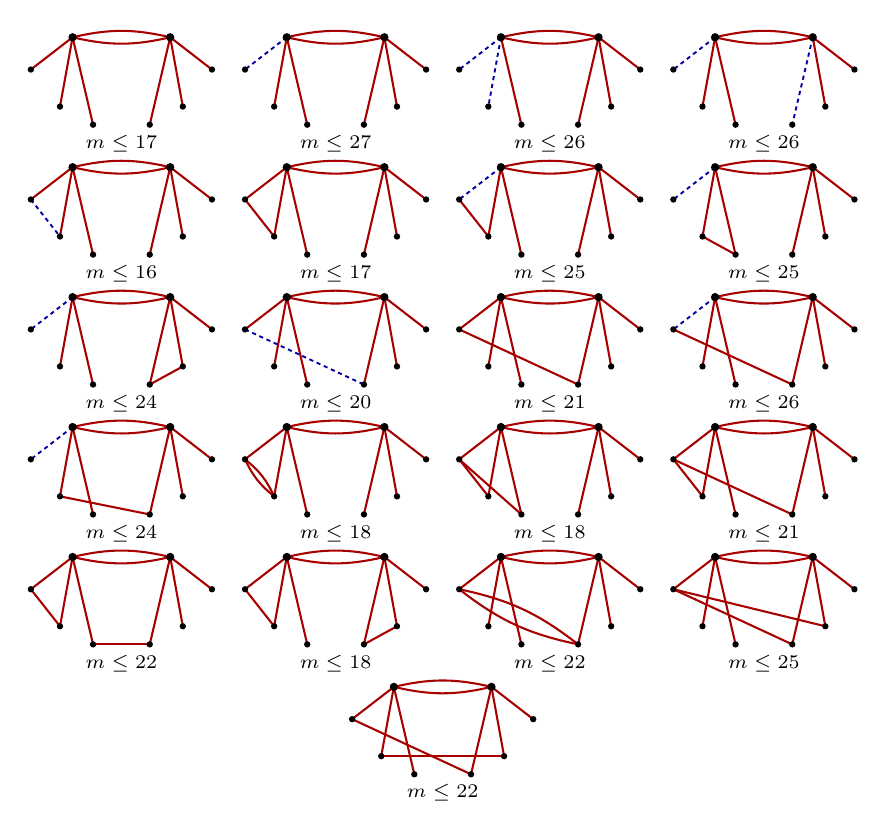
\begin{tikzpicture}[font=\scriptsize,
sc marked/.style={draw=red!65!black,line width=.75pt},
sc unmarked/.style={draw=blue!65!black,line width=.68pt,dash pattern=on 1.5pt off 1.35pt}]
\begin{scope}[shift={(-4.08,0)}]
\coordinate (u) at (-0.62,0.35);
\coordinate (v) at (0.62,0.35);
\coordinate (a0) at (-1.15,-0.06);
\coordinate (a1) at (-0.78,-0.53);
\coordinate (a2) at (-0.36,-0.76);
\coordinate (a3) at (0.36,-0.76);
\coordinate (a4) at (0.78,-0.53);
\coordinate (a5) at (1.15,-0.06);
\draw[sc marked] (u) to[bend left=13] (v);
\draw[sc marked] (u) to[bend right=13] (v);
\draw[sc marked] (u) -- (a0);
\draw[sc marked] (u) -- (a1);
\draw[sc marked] (u) -- (a2);
\draw[sc marked] (v) -- (a3);
\draw[sc marked] (v) -- (a4);
\draw[sc marked] (v) -- (a5);
\fill (u) circle[radius=1.5pt];
\fill (v) circle[radius=1.5pt];
\fill (a0) circle[radius=1.15pt];
\fill (a1) circle[radius=1.15pt];
\fill (a2) circle[radius=1.15pt];
\fill (a3) circle[radius=1.15pt];
\fill (a4) circle[radius=1.15pt];
\fill (a5) circle[radius=1.15pt];
\node[anchor=north,inner sep=1pt] at (0,-.85) {\(m\leq 17\)};
\end{scope}
\begin{scope}[shift={(-1.36,0)}]
\coordinate (u) at (-0.62,0.35);
\coordinate (v) at (0.62,0.35);
\coordinate (a0) at (-1.15,-0.06);
\coordinate (a1) at (-0.78,-0.53);
\coordinate (a2) at (-0.36,-0.76);
\coordinate (a3) at (0.36,-0.76);
\coordinate (a4) at (0.78,-0.53);
\coordinate (a5) at (1.15,-0.06);
\draw[sc marked] (u) to[bend left=13] (v);
\draw[sc marked] (u) to[bend right=13] (v);
\draw[sc unmarked] (u) -- (a0);
\draw[sc marked] (u) -- (a1);
\draw[sc marked] (u) -- (a2);
\draw[sc marked] (v) -- (a3);
\draw[sc marked] (v) -- (a4);
\draw[sc marked] (v) -- (a5);
\fill (u) circle[radius=1.5pt];
\fill (v) circle[radius=1.5pt];
\fill (a0) circle[radius=1.15pt];
\fill (a1) circle[radius=1.15pt];
\fill (a2) circle[radius=1.15pt];
\fill (a3) circle[radius=1.15pt];
\fill (a4) circle[radius=1.15pt];
\fill (a5) circle[radius=1.15pt];
\node[anchor=north,inner sep=1pt] at (0,-.85) {\(m\leq 27\)};
\end{scope}
\begin{scope}[shift={(1.36,0)}]
\coordinate (u) at (-0.62,0.35);
\coordinate (v) at (0.62,0.35);
\coordinate (a0) at (-1.15,-0.06);
\coordinate (a1) at (-0.78,-0.53);
\coordinate (a2) at (-0.36,-0.76);
\coordinate (a3) at (0.36,-0.76);
\coordinate (a4) at (0.78,-0.53);
\coordinate (a5) at (1.15,-0.06);
\draw[sc marked] (u) to[bend left=13] (v);
\draw[sc marked] (u) to[bend right=13] (v);
\draw[sc unmarked] (u) -- (a0);
\draw[sc unmarked] (u) -- (a1);
\draw[sc marked] (u) -- (a2);
\draw[sc marked] (v) -- (a3);
\draw[sc marked] (v) -- (a4);
\draw[sc marked] (v) -- (a5);
\fill (u) circle[radius=1.5pt];
\fill (v) circle[radius=1.5pt];
\fill (a0) circle[radius=1.15pt];
\fill (a1) circle[radius=1.15pt];
\fill (a2) circle[radius=1.15pt];
\fill (a3) circle[radius=1.15pt];
\fill (a4) circle[radius=1.15pt];
\fill (a5) circle[radius=1.15pt];
\node[anchor=north,inner sep=1pt] at (0,-.85) {\(m\leq 26\)};
\end{scope}
\begin{scope}[shift={(4.08,0)}]
\coordinate (u) at (-0.62,0.35);
\coordinate (v) at (0.62,0.35);
\coordinate (a0) at (-1.15,-0.06);
\coordinate (a1) at (-0.78,-0.53);
\coordinate (a2) at (-0.36,-0.76);
\coordinate (a3) at (0.36,-0.76);
\coordinate (a4) at (0.78,-0.53);
\coordinate (a5) at (1.15,-0.06);
\draw[sc marked] (u) to[bend left=13] (v);
\draw[sc marked] (u) to[bend right=13] (v);
\draw[sc unmarked] (u) -- (a0);
\draw[sc marked] (u) -- (a1);
\draw[sc marked] (u) -- (a2);
\draw[sc unmarked] (v) -- (a3);
\draw[sc marked] (v) -- (a4);
\draw[sc marked] (v) -- (a5);
\fill (u) circle[radius=1.5pt];
\fill (v) circle[radius=1.5pt];
\fill (a0) circle[radius=1.15pt];
\fill (a1) circle[radius=1.15pt];
\fill (a2) circle[radius=1.15pt];
\fill (a3) circle[radius=1.15pt];
\fill (a4) circle[radius=1.15pt];
\fill (a5) circle[radius=1.15pt];
\node[anchor=north,inner sep=1pt] at (0,-.85) {\(m\leq 26\)};
\end{scope}
\begin{scope}[shift={(-4.08,-1.65)}]
\coordinate (u) at (-0.62,0.35);
\coordinate (v) at (0.62,0.35);
\coordinate (a0) at (-1.15,-0.06);
\coordinate (a1) at (-0.78,-0.53);
\coordinate (a2) at (-0.36,-0.76);
\coordinate (a3) at (0.36,-0.76);
\coordinate (a4) at (0.78,-0.53);
\coordinate (a5) at (1.15,-0.06);
\draw[sc marked] (u) to[bend left=13] (v);
\draw[sc marked] (u) to[bend right=13] (v);
\draw[sc marked] (u) -- (a0);
\draw[sc marked] (u) -- (a1);
\draw[sc marked] (u) -- (a2);
\draw[sc marked] (v) -- (a3);
\draw[sc marked] (v) -- (a4);
\draw[sc marked] (v) -- (a5);
\draw[sc unmarked] (a0) -- (a1);
\fill (u) circle[radius=1.5pt];
\fill (v) circle[radius=1.5pt];
\fill (a0) circle[radius=1.15pt];
\fill (a1) circle[radius=1.15pt];
\fill (a2) circle[radius=1.15pt];
\fill (a3) circle[radius=1.15pt];
\fill (a4) circle[radius=1.15pt];
\fill (a5) circle[radius=1.15pt];
\node[anchor=north,inner sep=1pt] at (0,-.85) {\(m\leq 16\)};
\end{scope}
\begin{scope}[shift={(-1.36,-1.65)}]
\coordinate (u) at (-0.62,0.35);
\coordinate (v) at (0.62,0.35);
\coordinate (a0) at (-1.15,-0.06);
\coordinate (a1) at (-0.78,-0.53);
\coordinate (a2) at (-0.36,-0.76);
\coordinate (a3) at (0.36,-0.76);
\coordinate (a4) at (0.78,-0.53);
\coordinate (a5) at (1.15,-0.06);
\draw[sc marked] (u) to[bend left=13] (v);
\draw[sc marked] (u) to[bend right=13] (v);
\draw[sc marked] (u) -- (a0);
\draw[sc marked] (u) -- (a1);
\draw[sc marked] (u) -- (a2);
\draw[sc marked] (v) -- (a3);
\draw[sc marked] (v) -- (a4);
\draw[sc marked] (v) -- (a5);
\draw[sc marked] (a0) -- (a1);
\fill (u) circle[radius=1.5pt];
\fill (v) circle[radius=1.5pt];
\fill (a0) circle[radius=1.15pt];
\fill (a1) circle[radius=1.15pt];
\fill (a2) circle[radius=1.15pt];
\fill (a3) circle[radius=1.15pt];
\fill (a4) circle[radius=1.15pt];
\fill (a5) circle[radius=1.15pt];
\node[anchor=north,inner sep=1pt] at (0,-.85) {\(m\leq 17\)};
\end{scope}
\begin{scope}[shift={(1.36,-1.65)}]
\coordinate (u) at (-0.62,0.35);
\coordinate (v) at (0.62,0.35);
\coordinate (a0) at (-1.15,-0.06);
\coordinate (a1) at (-0.78,-0.53);
\coordinate (a2) at (-0.36,-0.76);
\coordinate (a3) at (0.36,-0.76);
\coordinate (a4) at (0.78,-0.53);
\coordinate (a5) at (1.15,-0.06);
\draw[sc marked] (u) to[bend left=13] (v);
\draw[sc marked] (u) to[bend right=13] (v);
\draw[sc unmarked] (u) -- (a0);
\draw[sc marked] (u) -- (a1);
\draw[sc marked] (u) -- (a2);
\draw[sc marked] (v) -- (a3);
\draw[sc marked] (v) -- (a4);
\draw[sc marked] (v) -- (a5);
\draw[sc marked] (a0) -- (a1);
\fill (u) circle[radius=1.5pt];
\fill (v) circle[radius=1.5pt];
\fill (a0) circle[radius=1.15pt];
\fill (a1) circle[radius=1.15pt];
\fill (a2) circle[radius=1.15pt];
\fill (a3) circle[radius=1.15pt];
\fill (a4) circle[radius=1.15pt];
\fill (a5) circle[radius=1.15pt];
\node[anchor=north,inner sep=1pt] at (0,-.85) {\(m\leq 25\)};
\end{scope}
\begin{scope}[shift={(4.08,-1.65)}]
\coordinate (u) at (-0.62,0.35);
\coordinate (v) at (0.62,0.35);
\coordinate (a0) at (-1.15,-0.06);
\coordinate (a1) at (-0.78,-0.53);
\coordinate (a2) at (-0.36,-0.76);
\coordinate (a3) at (0.36,-0.76);
\coordinate (a4) at (0.78,-0.53);
\coordinate (a5) at (1.15,-0.06);
\draw[sc marked] (u) to[bend left=13] (v);
\draw[sc marked] (u) to[bend right=13] (v);
\draw[sc unmarked] (u) -- (a0);
\draw[sc marked] (u) -- (a1);
\draw[sc marked] (u) -- (a2);
\draw[sc marked] (v) -- (a3);
\draw[sc marked] (v) -- (a4);
\draw[sc marked] (v) -- (a5);
\draw[sc marked] (a1) -- (a2);
\fill (u) circle[radius=1.5pt];
\fill (v) circle[radius=1.5pt];
\fill (a0) circle[radius=1.15pt];
\fill (a1) circle[radius=1.15pt];
\fill (a2) circle[radius=1.15pt];
\fill (a3) circle[radius=1.15pt];
\fill (a4) circle[radius=1.15pt];
\fill (a5) circle[radius=1.15pt];
\node[anchor=north,inner sep=1pt] at (0,-.85) {\(m\leq 25\)};
\end{scope}
\begin{scope}[shift={(-4.08,-3.3)}]
\coordinate (u) at (-0.62,0.35);
\coordinate (v) at (0.62,0.35);
\coordinate (a0) at (-1.15,-0.06);
\coordinate (a1) at (-0.78,-0.53);
\coordinate (a2) at (-0.36,-0.76);
\coordinate (a3) at (0.36,-0.76);
\coordinate (a4) at (0.78,-0.53);
\coordinate (a5) at (1.15,-0.06);
\draw[sc marked] (u) to[bend left=13] (v);
\draw[sc marked] (u) to[bend right=13] (v);
\draw[sc unmarked] (u) -- (a0);
\draw[sc marked] (u) -- (a1);
\draw[sc marked] (u) -- (a2);
\draw[sc marked] (v) -- (a3);
\draw[sc marked] (v) -- (a4);
\draw[sc marked] (v) -- (a5);
\draw[sc marked] (a3) -- (a4);
\fill (u) circle[radius=1.5pt];
\fill (v) circle[radius=1.5pt];
\fill (a0) circle[radius=1.15pt];
\fill (a1) circle[radius=1.15pt];
\fill (a2) circle[radius=1.15pt];
\fill (a3) circle[radius=1.15pt];
\fill (a4) circle[radius=1.15pt];
\fill (a5) circle[radius=1.15pt];
\node[anchor=north,inner sep=1pt] at (0,-.85) {\(m\leq 24\)};
\end{scope}
\begin{scope}[shift={(-1.36,-3.3)}]
\coordinate (u) at (-0.62,0.35);
\coordinate (v) at (0.62,0.35);
\coordinate (a0) at (-1.15,-0.06);
\coordinate (a1) at (-0.78,-0.53);
\coordinate (a2) at (-0.36,-0.76);
\coordinate (a3) at (0.36,-0.76);
\coordinate (a4) at (0.78,-0.53);
\coordinate (a5) at (1.15,-0.06);
\draw[sc marked] (u) to[bend left=13] (v);
\draw[sc marked] (u) to[bend right=13] (v);
\draw[sc marked] (u) -- (a0);
\draw[sc marked] (u) -- (a1);
\draw[sc marked] (u) -- (a2);
\draw[sc marked] (v) -- (a3);
\draw[sc marked] (v) -- (a4);
\draw[sc marked] (v) -- (a5);
\draw[sc unmarked] (a0) -- (a3);
\fill (u) circle[radius=1.5pt];
\fill (v) circle[radius=1.5pt];
\fill (a0) circle[radius=1.15pt];
\fill (a1) circle[radius=1.15pt];
\fill (a2) circle[radius=1.15pt];
\fill (a3) circle[radius=1.15pt];
\fill (a4) circle[radius=1.15pt];
\fill (a5) circle[radius=1.15pt];
\node[anchor=north,inner sep=1pt] at (0,-.85) {\(m\leq 20\)};
\end{scope}
\begin{scope}[shift={(1.36,-3.3)}]
\coordinate (u) at (-0.62,0.35);
\coordinate (v) at (0.62,0.35);
\coordinate (a0) at (-1.15,-0.06);
\coordinate (a1) at (-0.78,-0.53);
\coordinate (a2) at (-0.36,-0.76);
\coordinate (a3) at (0.36,-0.76);
\coordinate (a4) at (0.78,-0.53);
\coordinate (a5) at (1.15,-0.06);
\draw[sc marked] (u) to[bend left=13] (v);
\draw[sc marked] (u) to[bend right=13] (v);
\draw[sc marked] (u) -- (a0);
\draw[sc marked] (u) -- (a1);
\draw[sc marked] (u) -- (a2);
\draw[sc marked] (v) -- (a3);
\draw[sc marked] (v) -- (a4);
\draw[sc marked] (v) -- (a5);
\draw[sc marked] (a0) -- (a3);
\fill (u) circle[radius=1.5pt];
\fill (v) circle[radius=1.5pt];
\fill (a0) circle[radius=1.15pt];
\fill (a1) circle[radius=1.15pt];
\fill (a2) circle[radius=1.15pt];
\fill (a3) circle[radius=1.15pt];
\fill (a4) circle[radius=1.15pt];
\fill (a5) circle[radius=1.15pt];
\node[anchor=north,inner sep=1pt] at (0,-.85) {\(m\leq 21\)};
\end{scope}
\begin{scope}[shift={(4.08,-3.3)}]
\coordinate (u) at (-0.62,0.35);
\coordinate (v) at (0.62,0.35);
\coordinate (a0) at (-1.15,-0.06);
\coordinate (a1) at (-0.78,-0.53);
\coordinate (a2) at (-0.36,-0.76);
\coordinate (a3) at (0.36,-0.76);
\coordinate (a4) at (0.78,-0.53);
\coordinate (a5) at (1.15,-0.06);
\draw[sc marked] (u) to[bend left=13] (v);
\draw[sc marked] (u) to[bend right=13] (v);
\draw[sc unmarked] (u) -- (a0);
\draw[sc marked] (u) -- (a1);
\draw[sc marked] (u) -- (a2);
\draw[sc marked] (v) -- (a3);
\draw[sc marked] (v) -- (a4);
\draw[sc marked] (v) -- (a5);
\draw[sc marked] (a0) -- (a3);
\fill (u) circle[radius=1.5pt];
\fill (v) circle[radius=1.5pt];
\fill (a0) circle[radius=1.15pt];
\fill (a1) circle[radius=1.15pt];
\fill (a2) circle[radius=1.15pt];
\fill (a3) circle[radius=1.15pt];
\fill (a4) circle[radius=1.15pt];
\fill (a5) circle[radius=1.15pt];
\node[anchor=north,inner sep=1pt] at (0,-.85) {\(m\leq 26\)};
\end{scope}
\begin{scope}[shift={(-4.08,-4.95)}]
\coordinate (u) at (-0.62,0.35);
\coordinate (v) at (0.62,0.35);
\coordinate (a0) at (-1.15,-0.06);
\coordinate (a1) at (-0.78,-0.53);
\coordinate (a2) at (-0.36,-0.76);
\coordinate (a3) at (0.36,-0.76);
\coordinate (a4) at (0.78,-0.53);
\coordinate (a5) at (1.15,-0.06);
\draw[sc marked] (u) to[bend left=13] (v);
\draw[sc marked] (u) to[bend right=13] (v);
\draw[sc unmarked] (u) -- (a0);
\draw[sc marked] (u) -- (a1);
\draw[sc marked] (u) -- (a2);
\draw[sc marked] (v) -- (a3);
\draw[sc marked] (v) -- (a4);
\draw[sc marked] (v) -- (a5);
\draw[sc marked] (a1) -- (a3);
\fill (u) circle[radius=1.5pt];
\fill (v) circle[radius=1.5pt];
\fill (a0) circle[radius=1.15pt];
\fill (a1) circle[radius=1.15pt];
\fill (a2) circle[radius=1.15pt];
\fill (a3) circle[radius=1.15pt];
\fill (a4) circle[radius=1.15pt];
\fill (a5) circle[radius=1.15pt];
\node[anchor=north,inner sep=1pt] at (0,-.85) {\(m\leq 24\)};
\end{scope}
\begin{scope}[shift={(-1.36,-4.95)}]
\coordinate (u) at (-0.62,0.35);
\coordinate (v) at (0.62,0.35);
\coordinate (a0) at (-1.15,-0.06);
\coordinate (a1) at (-0.78,-0.53);
\coordinate (a2) at (-0.36,-0.76);
\coordinate (a3) at (0.36,-0.76);
\coordinate (a4) at (0.78,-0.53);
\coordinate (a5) at (1.15,-0.06);
\draw[sc marked] (u) to[bend left=13] (v);
\draw[sc marked] (u) to[bend right=13] (v);
\draw[sc marked] (u) -- (a0);
\draw[sc marked] (u) -- (a1);
\draw[sc marked] (u) -- (a2);
\draw[sc marked] (v) -- (a3);
\draw[sc marked] (v) -- (a4);
\draw[sc marked] (v) -- (a5);
\draw[sc marked] (a0) to[bend left=13] (a1);
\draw[sc marked] (a0) to[bend right=13] (a1);
\fill (u) circle[radius=1.5pt];
\fill (v) circle[radius=1.5pt];
\fill (a0) circle[radius=1.15pt];
\fill (a1) circle[radius=1.15pt];
\fill (a2) circle[radius=1.15pt];
\fill (a3) circle[radius=1.15pt];
\fill (a4) circle[radius=1.15pt];
\fill (a5) circle[radius=1.15pt];
\node[anchor=north,inner sep=1pt] at (0,-.85) {\(m\leq 18\)};
\end{scope}
\begin{scope}[shift={(1.36,-4.95)}]
\coordinate (u) at (-0.62,0.35);
\coordinate (v) at (0.62,0.35);
\coordinate (a0) at (-1.15,-0.06);
\coordinate (a1) at (-0.78,-0.53);
\coordinate (a2) at (-0.36,-0.76);
\coordinate (a3) at (0.36,-0.76);
\coordinate (a4) at (0.78,-0.53);
\coordinate (a5) at (1.15,-0.06);
\draw[sc marked] (u) to[bend left=13] (v);
\draw[sc marked] (u) to[bend right=13] (v);
\draw[sc marked] (u) -- (a0);
\draw[sc marked] (u) -- (a1);
\draw[sc marked] (u) -- (a2);
\draw[sc marked] (v) -- (a3);
\draw[sc marked] (v) -- (a4);
\draw[sc marked] (v) -- (a5);
\draw[sc marked] (a0) -- (a1);
\draw[sc marked] (a0) -- (a2);
\fill (u) circle[radius=1.5pt];
\fill (v) circle[radius=1.5pt];
\fill (a0) circle[radius=1.15pt];
\fill (a1) circle[radius=1.15pt];
\fill (a2) circle[radius=1.15pt];
\fill (a3) circle[radius=1.15pt];
\fill (a4) circle[radius=1.15pt];
\fill (a5) circle[radius=1.15pt];
\node[anchor=north,inner sep=1pt] at (0,-.85) {\(m\leq 18\)};
\end{scope}
\begin{scope}[shift={(4.08,-4.95)}]
\coordinate (u) at (-0.62,0.35);
\coordinate (v) at (0.62,0.35);
\coordinate (a0) at (-1.15,-0.06);
\coordinate (a1) at (-0.78,-0.53);
\coordinate (a2) at (-0.36,-0.76);
\coordinate (a3) at (0.36,-0.76);
\coordinate (a4) at (0.78,-0.53);
\coordinate (a5) at (1.15,-0.06);
\draw[sc marked] (u) to[bend left=13] (v);
\draw[sc marked] (u) to[bend right=13] (v);
\draw[sc marked] (u) -- (a0);
\draw[sc marked] (u) -- (a1);
\draw[sc marked] (u) -- (a2);
\draw[sc marked] (v) -- (a3);
\draw[sc marked] (v) -- (a4);
\draw[sc marked] (v) -- (a5);
\draw[sc marked] (a0) -- (a1);
\draw[sc marked] (a0) -- (a3);
\fill (u) circle[radius=1.5pt];
\fill (v) circle[radius=1.5pt];
\fill (a0) circle[radius=1.15pt];
\fill (a1) circle[radius=1.15pt];
\fill (a2) circle[radius=1.15pt];
\fill (a3) circle[radius=1.15pt];
\fill (a4) circle[radius=1.15pt];
\fill (a5) circle[radius=1.15pt];
\node[anchor=north,inner sep=1pt] at (0,-.85) {\(m\leq 21\)};
\end{scope}
\begin{scope}[shift={(-4.08,-6.6)}]
\coordinate (u) at (-0.62,0.35);
\coordinate (v) at (0.62,0.35);
\coordinate (a0) at (-1.15,-0.06);
\coordinate (a1) at (-0.78,-0.53);
\coordinate (a2) at (-0.36,-0.76);
\coordinate (a3) at (0.36,-0.76);
\coordinate (a4) at (0.78,-0.53);
\coordinate (a5) at (1.15,-0.06);
\draw[sc marked] (u) to[bend left=13] (v);
\draw[sc marked] (u) to[bend right=13] (v);
\draw[sc marked] (u) -- (a0);
\draw[sc marked] (u) -- (a1);
\draw[sc marked] (u) -- (a2);
\draw[sc marked] (v) -- (a3);
\draw[sc marked] (v) -- (a4);
\draw[sc marked] (v) -- (a5);
\draw[sc marked] (a0) -- (a1);
\draw[sc marked] (a2) -- (a3);
\fill (u) circle[radius=1.5pt];
\fill (v) circle[radius=1.5pt];
\fill (a0) circle[radius=1.15pt];
\fill (a1) circle[radius=1.15pt];
\fill (a2) circle[radius=1.15pt];
\fill (a3) circle[radius=1.15pt];
\fill (a4) circle[radius=1.15pt];
\fill (a5) circle[radius=1.15pt];
\node[anchor=north,inner sep=1pt] at (0,-.85) {\(m\leq 22\)};
\end{scope}
\begin{scope}[shift={(-1.36,-6.6)}]
\coordinate (u) at (-0.62,0.35);
\coordinate (v) at (0.62,0.35);
\coordinate (a0) at (-1.15,-0.06);
\coordinate (a1) at (-0.78,-0.53);
\coordinate (a2) at (-0.36,-0.76);
\coordinate (a3) at (0.36,-0.76);
\coordinate (a4) at (0.78,-0.53);
\coordinate (a5) at (1.15,-0.06);
\draw[sc marked] (u) to[bend left=13] (v);
\draw[sc marked] (u) to[bend right=13] (v);
\draw[sc marked] (u) -- (a0);
\draw[sc marked] (u) -- (a1);
\draw[sc marked] (u) -- (a2);
\draw[sc marked] (v) -- (a3);
\draw[sc marked] (v) -- (a4);
\draw[sc marked] (v) -- (a5);
\draw[sc marked] (a0) -- (a1);
\draw[sc marked] (a3) -- (a4);
\fill (u) circle[radius=1.5pt];
\fill (v) circle[radius=1.5pt];
\fill (a0) circle[radius=1.15pt];
\fill (a1) circle[radius=1.15pt];
\fill (a2) circle[radius=1.15pt];
\fill (a3) circle[radius=1.15pt];
\fill (a4) circle[radius=1.15pt];
\fill (a5) circle[radius=1.15pt];
\node[anchor=north,inner sep=1pt] at (0,-.85) {\(m\leq 18\)};
\end{scope}
\begin{scope}[shift={(1.36,-6.6)}]
\coordinate (u) at (-0.62,0.35);
\coordinate (v) at (0.62,0.35);
\coordinate (a0) at (-1.15,-0.06);
\coordinate (a1) at (-0.78,-0.53);
\coordinate (a2) at (-0.36,-0.76);
\coordinate (a3) at (0.36,-0.76);
\coordinate (a4) at (0.78,-0.53);
\coordinate (a5) at (1.15,-0.06);
\draw[sc marked] (u) to[bend left=13] (v);
\draw[sc marked] (u) to[bend right=13] (v);
\draw[sc marked] (u) -- (a0);
\draw[sc marked] (u) -- (a1);
\draw[sc marked] (u) -- (a2);
\draw[sc marked] (v) -- (a3);
\draw[sc marked] (v) -- (a4);
\draw[sc marked] (v) -- (a5);
\draw[sc marked] (a0) to[bend left=13] (a3);
\draw[sc marked] (a0) to[bend right=13] (a3);
\fill (u) circle[radius=1.5pt];
\fill (v) circle[radius=1.5pt];
\fill (a0) circle[radius=1.15pt];
\fill (a1) circle[radius=1.15pt];
\fill (a2) circle[radius=1.15pt];
\fill (a3) circle[radius=1.15pt];
\fill (a4) circle[radius=1.15pt];
\fill (a5) circle[radius=1.15pt];
\node[anchor=north,inner sep=1pt] at (0,-.85) {\(m\leq 22\)};
\end{scope}
\begin{scope}[shift={(4.08,-6.6)}]
\coordinate (u) at (-0.62,0.35);
\coordinate (v) at (0.62,0.35);
\coordinate (a0) at (-1.15,-0.06);
\coordinate (a1) at (-0.78,-0.53);
\coordinate (a2) at (-0.36,-0.76);
\coordinate (a3) at (0.36,-0.76);
\coordinate (a4) at (0.78,-0.53);
\coordinate (a5) at (1.15,-0.06);
\draw[sc marked] (u) to[bend left=13] (v);
\draw[sc marked] (u) to[bend right=13] (v);
\draw[sc marked] (u) -- (a0);
\draw[sc marked] (u) -- (a1);
\draw[sc marked] (u) -- (a2);
\draw[sc marked] (v) -- (a3);
\draw[sc marked] (v) -- (a4);
\draw[sc marked] (v) -- (a5);
\draw[sc marked] (a0) -- (a3);
\draw[sc marked] (a0) -- (a4);
\fill (u) circle[radius=1.5pt];
\fill (v) circle[radius=1.5pt];
\fill (a0) circle[radius=1.15pt];
\fill (a1) circle[radius=1.15pt];
\fill (a2) circle[radius=1.15pt];
\fill (a3) circle[radius=1.15pt];
\fill (a4) circle[radius=1.15pt];
\fill (a5) circle[radius=1.15pt];
\node[anchor=north,inner sep=1pt] at (0,-.85) {\(m\leq 25\)};
\end{scope}
\begin{scope}[shift={(0,-8.25)}]
\coordinate (u) at (-0.62,0.35);
\coordinate (v) at (0.62,0.35);
\coordinate (a0) at (-1.15,-0.06);
\coordinate (a1) at (-0.78,-0.53);
\coordinate (a2) at (-0.36,-0.76);
\coordinate (a3) at (0.36,-0.76);
\coordinate (a4) at (0.78,-0.53);
\coordinate (a5) at (1.15,-0.06);
\draw[sc marked] (u) to[bend left=13] (v);
\draw[sc marked] (u) to[bend right=13] (v);
\draw[sc marked] (u) -- (a0);
\draw[sc marked] (u) -- (a1);
\draw[sc marked] (u) -- (a2);
\draw[sc marked] (v) -- (a3);
\draw[sc marked] (v) -- (a4);
\draw[sc marked] (v) -- (a5);
\draw[sc marked] (a0) -- (a3);
\draw[sc marked] (a1) -- (a4);
\fill (u) circle[radius=1.5pt];
\fill (v) circle[radius=1.5pt];
\fill (a0) circle[radius=1.15pt];
\fill (a1) circle[radius=1.15pt];
\fill (a2) circle[radius=1.15pt];
\fill (a3) circle[radius=1.15pt];
\fill (a4) circle[radius=1.15pt];
\fill (a5) circle[radius=1.15pt];
\node[anchor=north,inner sep=1pt] at (0,-.85) {\(m\leq 22\)};
\end{scope}
\end{tikzpicture}
\caption{The 21 root configurations at degree five and their upper bounds on $m$. The two upper vertices are the roots. Solid edges are marked and dashed edges are unmarked. Two arcs between a pair of vertices denote two copies.}
\label{fig:finite-five-spokes}
\end{figure}

\FloatBarrier

At $D=7$, we have $m=59$. Equation
\eqref{eq:multi-root-pair-budget} excludes $k\ge4$. If
$k=3$, then $q\le8$, and its second line forces $q=8$,
$d_H(a)=7$ for every $a\in A$, and $e_H(A)=0$.
All edges incident with $A$ are marked, so $G[A]$ has no
edges. The two roots have disjoint sets of four neighbors in
$A$. A marked edge from one set to $x\in W$ forces $x$ to
be adjacent to all four vertices of the other set, by comparison
with their spokes. These four edges at $x$ are also marked.
Comparing one of them with the spokes on the first side forces
four more neighbors at $x$, exceeding the degree bound.
Thus every repeated marked pair has multiplicity two.

Fix such a pair as the root pair. Equation
\eqref{eq:multi-root-pair-budget} gives $q\in\{9,10\}$.
Let $T$ count spokes with multiplicity, $p$ count the
unmarked spokes, and $i_m$ and $i_u$ count marked and
unmarked edges within $A$. Let $m_\times$ and $U$ count
marked and unmarked edges between $A$ and $W$, respectively,
and put $\ell=\sum_{a\in A}(7-d_G(a))$. Counting the
marked edges and summing the degrees on $A$ gives
\begin{equation}\label{eq:multi-seven-counts}
 57=T-p+i_m+m_\times,\qquad
 \ell+p+i_m+2i_u+U=7q-57.
\end{equation}
As $T,q\le10$, these equations imply $m_\times\ge34+2p$.

To bound $w=|W|$, assign each vertex in $W$ to one of its
marked neighbors in $A$. Let $n_a$ be the number assigned
to $a\in A$. Write $J$ for the simple support of $G[A]$
and $D_A=m_\times+U$ for the number of edges between $A$
and $W$. If $a,b$ are nonadjacent in $J$, vertices $x,y$
assigned to $a,b$, respectively, give disjoint marked edges
$ax$ and $by$. At least one of $xy,ay,bx$ must be an edge of $G$. Write $d_G(a,W)$ for the number of edges from $a$ to $W$,
counted with multiplicity. The number of such unordered pairs
$\{x,y\}$ is at most $|E(G[W])|+\sum_a n_a(d_G(a,W)-n_a)$. Using
$d_G(a,W)\le6-d_J(a)$ and $2|E(G[W])|\le7w-D_A$ gives
\[
 w^2+\sum_a n_a^2+2\sum_{ab\in E(J)}(n_a+n_b-n_an_b)
 \le 19w-D_A.
\]
The inequality $2n_an_b\le n_a^2+n_b^2$ bounds the
left side from below by $w^2+\sum_a[n_a^2+d_J(a)n_a(2-n_a)]$.
Each summand is nonnegative. For $n_a\ge3$, this follows
from $d_J(a)\le6-n_a$, which bounds the summand below
by $n_a(n_a-3)(n_a-4)$. Since $D_A\ge34$, we obtain
$w\le17$. If $w=17$, both inequalities are equalities, so
every positive $n_a$ is three or four, every vertex with
$n_a=3$ has degree three in $J$, and the endpoints of each
edge of $J$ have equal group sizes. The group sizes must
then be $3,3,3,4,4$. Each of the three vertices with group
size three has at most two possible neighbors in $J$, a
contradiction. Hence $w\le16$.

Delete $u,v$ from the host and mark only the edges between
$A$ and $W$. These edges still form a strong clique. The
marked graph is bipartite, and the host can have edges within
either side. The host degrees on the two sides are at most
six and seven. Thus the Ore-degree of the bipartite marked
subgraph in the host after deletion is at most 13.
Applying the recurrence based on \eqref{eq:finite-bipartite-root-count}
gives $m_\times\le48$ for Ore-degree at most 13 and
$m_\times\le41$ for Ore-degree at most 12.

From \eqref{eq:multi-seven-counts} we have $i_m\leq7q-57-p$ and hence
$m_\times\geq114-T-7q+2p$. Since $T\leq10$ and $m_\times\leq48$, this
gives $p\le7$ at $q=10$ and $p\le3$ at $q=9$. At $q=10$ both roots
have five distinct neighbors outside $\{u,v\}$, and their two neighbor
sets are disjoint. All ten spokes are single. The numbers of marked
spokes at the roots determine the configuration up to interchanging
the roots and permuting their neighbors.
\textbf{Figure~\ref{fig:finite-seven-disjoint}} shows the 17 possibilities.

\begin{figure}[htbp]
\centering
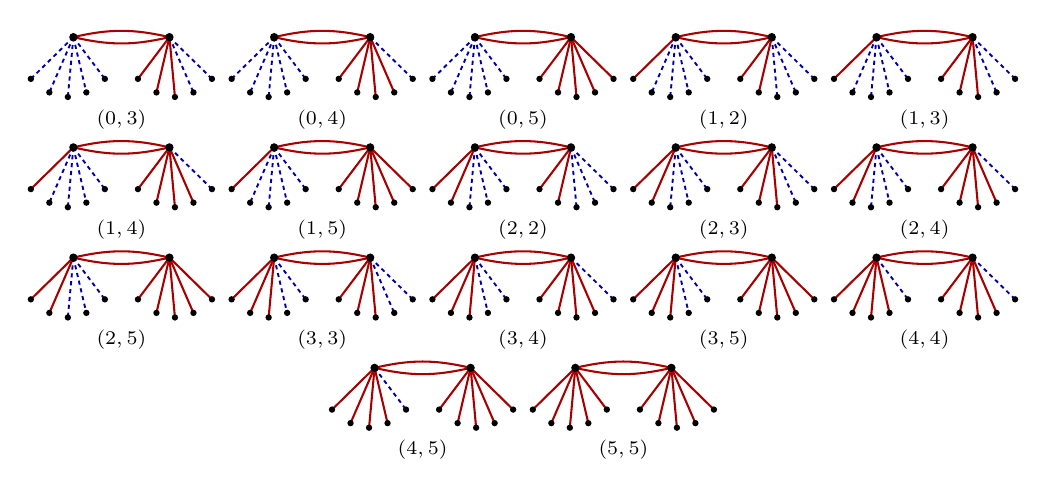
\begin{tikzpicture}[font=\scriptsize,
sc marked/.style={draw=red!65!black,line width=.75pt},
sc unmarked/.style={draw=blue!65!black,line width=.68pt,dash pattern=on 1.5pt off 1.35pt}]
\begin{scope}[shift={(-5.1,0)}]
\coordinate (u) at (-0.61,0.03);
\coordinate (v) at (0.61,0.03);
\coordinate (u0) at (-1.15,-0.5);
\coordinate (u1) at (-0.915,-0.672);
\coordinate (u2) at (-0.68,-0.73);
\coordinate (u3) at (-0.445,-0.672);
\coordinate (u4) at (-0.21,-0.5);
\coordinate (v0) at (0.21,-0.5);
\coordinate (v1) at (0.445,-0.672);
\coordinate (v2) at (0.68,-0.73);
\coordinate (v3) at (0.915,-0.672);
\coordinate (v4) at (1.15,-0.5);
\draw[sc marked] (u) to[bend left=13] (v);
\draw[sc marked] (u) to[bend right=13] (v);
\draw[sc unmarked] (u) -- (u0);
\draw[sc unmarked] (u) -- (u1);
\draw[sc unmarked] (u) -- (u2);
\draw[sc unmarked] (u) -- (u3);
\draw[sc unmarked] (u) -- (u4);
\draw[sc marked] (v) -- (v0);
\draw[sc marked] (v) -- (v1);
\draw[sc marked] (v) -- (v2);
\draw[sc unmarked] (v) -- (v3);
\draw[sc unmarked] (v) -- (v4);
\fill (u) circle[radius=1.5pt];
\fill (v) circle[radius=1.5pt];
\fill (u0) circle[radius=1.15pt];
\fill (u1) circle[radius=1.15pt];
\fill (u2) circle[radius=1.15pt];
\fill (u3) circle[radius=1.15pt];
\fill (u4) circle[radius=1.15pt];
\fill (v0) circle[radius=1.15pt];
\fill (v1) circle[radius=1.15pt];
\fill (v2) circle[radius=1.15pt];
\fill (v3) circle[radius=1.15pt];
\fill (v4) circle[radius=1.15pt];
\node[anchor=north,inner sep=1pt] at (0,-.85) {\((0,3)\)};
\end{scope}
\begin{scope}[shift={(-2.55,0)}]
\coordinate (u) at (-0.61,0.03);
\coordinate (v) at (0.61,0.03);
\coordinate (u0) at (-1.15,-0.5);
\coordinate (u1) at (-0.915,-0.672);
\coordinate (u2) at (-0.68,-0.73);
\coordinate (u3) at (-0.445,-0.672);
\coordinate (u4) at (-0.21,-0.5);
\coordinate (v0) at (0.21,-0.5);
\coordinate (v1) at (0.445,-0.672);
\coordinate (v2) at (0.68,-0.73);
\coordinate (v3) at (0.915,-0.672);
\coordinate (v4) at (1.15,-0.5);
\draw[sc marked] (u) to[bend left=13] (v);
\draw[sc marked] (u) to[bend right=13] (v);
\draw[sc unmarked] (u) -- (u0);
\draw[sc unmarked] (u) -- (u1);
\draw[sc unmarked] (u) -- (u2);
\draw[sc unmarked] (u) -- (u3);
\draw[sc unmarked] (u) -- (u4);
\draw[sc marked] (v) -- (v0);
\draw[sc marked] (v) -- (v1);
\draw[sc marked] (v) -- (v2);
\draw[sc marked] (v) -- (v3);
\draw[sc unmarked] (v) -- (v4);
\fill (u) circle[radius=1.5pt];
\fill (v) circle[radius=1.5pt];
\fill (u0) circle[radius=1.15pt];
\fill (u1) circle[radius=1.15pt];
\fill (u2) circle[radius=1.15pt];
\fill (u3) circle[radius=1.15pt];
\fill (u4) circle[radius=1.15pt];
\fill (v0) circle[radius=1.15pt];
\fill (v1) circle[radius=1.15pt];
\fill (v2) circle[radius=1.15pt];
\fill (v3) circle[radius=1.15pt];
\fill (v4) circle[radius=1.15pt];
\node[anchor=north,inner sep=1pt] at (0,-.85) {\((0,4)\)};
\end{scope}
\begin{scope}[shift={(0,0)}]
\coordinate (u) at (-0.61,0.03);
\coordinate (v) at (0.61,0.03);
\coordinate (u0) at (-1.15,-0.5);
\coordinate (u1) at (-0.915,-0.672);
\coordinate (u2) at (-0.68,-0.73);
\coordinate (u3) at (-0.445,-0.672);
\coordinate (u4) at (-0.21,-0.5);
\coordinate (v0) at (0.21,-0.5);
\coordinate (v1) at (0.445,-0.672);
\coordinate (v2) at (0.68,-0.73);
\coordinate (v3) at (0.915,-0.672);
\coordinate (v4) at (1.15,-0.5);
\draw[sc marked] (u) to[bend left=13] (v);
\draw[sc marked] (u) to[bend right=13] (v);
\draw[sc unmarked] (u) -- (u0);
\draw[sc unmarked] (u) -- (u1);
\draw[sc unmarked] (u) -- (u2);
\draw[sc unmarked] (u) -- (u3);
\draw[sc unmarked] (u) -- (u4);
\draw[sc marked] (v) -- (v0);
\draw[sc marked] (v) -- (v1);
\draw[sc marked] (v) -- (v2);
\draw[sc marked] (v) -- (v3);
\draw[sc marked] (v) -- (v4);
\fill (u) circle[radius=1.5pt];
\fill (v) circle[radius=1.5pt];
\fill (u0) circle[radius=1.15pt];
\fill (u1) circle[radius=1.15pt];
\fill (u2) circle[radius=1.15pt];
\fill (u3) circle[radius=1.15pt];
\fill (u4) circle[radius=1.15pt];
\fill (v0) circle[radius=1.15pt];
\fill (v1) circle[radius=1.15pt];
\fill (v2) circle[radius=1.15pt];
\fill (v3) circle[radius=1.15pt];
\fill (v4) circle[radius=1.15pt];
\node[anchor=north,inner sep=1pt] at (0,-.85) {\((0,5)\)};
\end{scope}
\begin{scope}[shift={(2.55,0)}]
\coordinate (u) at (-0.61,0.03);
\coordinate (v) at (0.61,0.03);
\coordinate (u0) at (-1.15,-0.5);
\coordinate (u1) at (-0.915,-0.672);
\coordinate (u2) at (-0.68,-0.73);
\coordinate (u3) at (-0.445,-0.672);
\coordinate (u4) at (-0.21,-0.5);
\coordinate (v0) at (0.21,-0.5);
\coordinate (v1) at (0.445,-0.672);
\coordinate (v2) at (0.68,-0.73);
\coordinate (v3) at (0.915,-0.672);
\coordinate (v4) at (1.15,-0.5);
\draw[sc marked] (u) to[bend left=13] (v);
\draw[sc marked] (u) to[bend right=13] (v);
\draw[sc marked] (u) -- (u0);
\draw[sc unmarked] (u) -- (u1);
\draw[sc unmarked] (u) -- (u2);
\draw[sc unmarked] (u) -- (u3);
\draw[sc unmarked] (u) -- (u4);
\draw[sc marked] (v) -- (v0);
\draw[sc marked] (v) -- (v1);
\draw[sc unmarked] (v) -- (v2);
\draw[sc unmarked] (v) -- (v3);
\draw[sc unmarked] (v) -- (v4);
\fill (u) circle[radius=1.5pt];
\fill (v) circle[radius=1.5pt];
\fill (u0) circle[radius=1.15pt];
\fill (u1) circle[radius=1.15pt];
\fill (u2) circle[radius=1.15pt];
\fill (u3) circle[radius=1.15pt];
\fill (u4) circle[radius=1.15pt];
\fill (v0) circle[radius=1.15pt];
\fill (v1) circle[radius=1.15pt];
\fill (v2) circle[radius=1.15pt];
\fill (v3) circle[radius=1.15pt];
\fill (v4) circle[radius=1.15pt];
\node[anchor=north,inner sep=1pt] at (0,-.85) {\((1,2)\)};
\end{scope}
\begin{scope}[shift={(5.1,0)}]
\coordinate (u) at (-0.61,0.03);
\coordinate (v) at (0.61,0.03);
\coordinate (u0) at (-1.15,-0.5);
\coordinate (u1) at (-0.915,-0.672);
\coordinate (u2) at (-0.68,-0.73);
\coordinate (u3) at (-0.445,-0.672);
\coordinate (u4) at (-0.21,-0.5);
\coordinate (v0) at (0.21,-0.5);
\coordinate (v1) at (0.445,-0.672);
\coordinate (v2) at (0.68,-0.73);
\coordinate (v3) at (0.915,-0.672);
\coordinate (v4) at (1.15,-0.5);
\draw[sc marked] (u) to[bend left=13] (v);
\draw[sc marked] (u) to[bend right=13] (v);
\draw[sc marked] (u) -- (u0);
\draw[sc unmarked] (u) -- (u1);
\draw[sc unmarked] (u) -- (u2);
\draw[sc unmarked] (u) -- (u3);
\draw[sc unmarked] (u) -- (u4);
\draw[sc marked] (v) -- (v0);
\draw[sc marked] (v) -- (v1);
\draw[sc marked] (v) -- (v2);
\draw[sc unmarked] (v) -- (v3);
\draw[sc unmarked] (v) -- (v4);
\fill (u) circle[radius=1.5pt];
\fill (v) circle[radius=1.5pt];
\fill (u0) circle[radius=1.15pt];
\fill (u1) circle[radius=1.15pt];
\fill (u2) circle[radius=1.15pt];
\fill (u3) circle[radius=1.15pt];
\fill (u4) circle[radius=1.15pt];
\fill (v0) circle[radius=1.15pt];
\fill (v1) circle[radius=1.15pt];
\fill (v2) circle[radius=1.15pt];
\fill (v3) circle[radius=1.15pt];
\fill (v4) circle[radius=1.15pt];
\node[anchor=north,inner sep=1pt] at (0,-.85) {\((1,3)\)};
\end{scope}
\begin{scope}[shift={(-5.1,-1.4)}]
\coordinate (u) at (-0.61,0.03);
\coordinate (v) at (0.61,0.03);
\coordinate (u0) at (-1.15,-0.5);
\coordinate (u1) at (-0.915,-0.672);
\coordinate (u2) at (-0.68,-0.73);
\coordinate (u3) at (-0.445,-0.672);
\coordinate (u4) at (-0.21,-0.5);
\coordinate (v0) at (0.21,-0.5);
\coordinate (v1) at (0.445,-0.672);
\coordinate (v2) at (0.68,-0.73);
\coordinate (v3) at (0.915,-0.672);
\coordinate (v4) at (1.15,-0.5);
\draw[sc marked] (u) to[bend left=13] (v);
\draw[sc marked] (u) to[bend right=13] (v);
\draw[sc marked] (u) -- (u0);
\draw[sc unmarked] (u) -- (u1);
\draw[sc unmarked] (u) -- (u2);
\draw[sc unmarked] (u) -- (u3);
\draw[sc unmarked] (u) -- (u4);
\draw[sc marked] (v) -- (v0);
\draw[sc marked] (v) -- (v1);
\draw[sc marked] (v) -- (v2);
\draw[sc marked] (v) -- (v3);
\draw[sc unmarked] (v) -- (v4);
\fill (u) circle[radius=1.5pt];
\fill (v) circle[radius=1.5pt];
\fill (u0) circle[radius=1.15pt];
\fill (u1) circle[radius=1.15pt];
\fill (u2) circle[radius=1.15pt];
\fill (u3) circle[radius=1.15pt];
\fill (u4) circle[radius=1.15pt];
\fill (v0) circle[radius=1.15pt];
\fill (v1) circle[radius=1.15pt];
\fill (v2) circle[radius=1.15pt];
\fill (v3) circle[radius=1.15pt];
\fill (v4) circle[radius=1.15pt];
\node[anchor=north,inner sep=1pt] at (0,-.85) {\((1,4)\)};
\end{scope}
\begin{scope}[shift={(-2.55,-1.4)}]
\coordinate (u) at (-0.61,0.03);
\coordinate (v) at (0.61,0.03);
\coordinate (u0) at (-1.15,-0.5);
\coordinate (u1) at (-0.915,-0.672);
\coordinate (u2) at (-0.68,-0.73);
\coordinate (u3) at (-0.445,-0.672);
\coordinate (u4) at (-0.21,-0.5);
\coordinate (v0) at (0.21,-0.5);
\coordinate (v1) at (0.445,-0.672);
\coordinate (v2) at (0.68,-0.73);
\coordinate (v3) at (0.915,-0.672);
\coordinate (v4) at (1.15,-0.5);
\draw[sc marked] (u) to[bend left=13] (v);
\draw[sc marked] (u) to[bend right=13] (v);
\draw[sc marked] (u) -- (u0);
\draw[sc unmarked] (u) -- (u1);
\draw[sc unmarked] (u) -- (u2);
\draw[sc unmarked] (u) -- (u3);
\draw[sc unmarked] (u) -- (u4);
\draw[sc marked] (v) -- (v0);
\draw[sc marked] (v) -- (v1);
\draw[sc marked] (v) -- (v2);
\draw[sc marked] (v) -- (v3);
\draw[sc marked] (v) -- (v4);
\fill (u) circle[radius=1.5pt];
\fill (v) circle[radius=1.5pt];
\fill (u0) circle[radius=1.15pt];
\fill (u1) circle[radius=1.15pt];
\fill (u2) circle[radius=1.15pt];
\fill (u3) circle[radius=1.15pt];
\fill (u4) circle[radius=1.15pt];
\fill (v0) circle[radius=1.15pt];
\fill (v1) circle[radius=1.15pt];
\fill (v2) circle[radius=1.15pt];
\fill (v3) circle[radius=1.15pt];
\fill (v4) circle[radius=1.15pt];
\node[anchor=north,inner sep=1pt] at (0,-.85) {\((1,5)\)};
\end{scope}
\begin{scope}[shift={(0,-1.4)}]
\coordinate (u) at (-0.61,0.03);
\coordinate (v) at (0.61,0.03);
\coordinate (u0) at (-1.15,-0.5);
\coordinate (u1) at (-0.915,-0.672);
\coordinate (u2) at (-0.68,-0.73);
\coordinate (u3) at (-0.445,-0.672);
\coordinate (u4) at (-0.21,-0.5);
\coordinate (v0) at (0.21,-0.5);
\coordinate (v1) at (0.445,-0.672);
\coordinate (v2) at (0.68,-0.73);
\coordinate (v3) at (0.915,-0.672);
\coordinate (v4) at (1.15,-0.5);
\draw[sc marked] (u) to[bend left=13] (v);
\draw[sc marked] (u) to[bend right=13] (v);
\draw[sc marked] (u) -- (u0);
\draw[sc marked] (u) -- (u1);
\draw[sc unmarked] (u) -- (u2);
\draw[sc unmarked] (u) -- (u3);
\draw[sc unmarked] (u) -- (u4);
\draw[sc marked] (v) -- (v0);
\draw[sc marked] (v) -- (v1);
\draw[sc unmarked] (v) -- (v2);
\draw[sc unmarked] (v) -- (v3);
\draw[sc unmarked] (v) -- (v4);
\fill (u) circle[radius=1.5pt];
\fill (v) circle[radius=1.5pt];
\fill (u0) circle[radius=1.15pt];
\fill (u1) circle[radius=1.15pt];
\fill (u2) circle[radius=1.15pt];
\fill (u3) circle[radius=1.15pt];
\fill (u4) circle[radius=1.15pt];
\fill (v0) circle[radius=1.15pt];
\fill (v1) circle[radius=1.15pt];
\fill (v2) circle[radius=1.15pt];
\fill (v3) circle[radius=1.15pt];
\fill (v4) circle[radius=1.15pt];
\node[anchor=north,inner sep=1pt] at (0,-.85) {\((2,2)\)};
\end{scope}
\begin{scope}[shift={(2.55,-1.4)}]
\coordinate (u) at (-0.61,0.03);
\coordinate (v) at (0.61,0.03);
\coordinate (u0) at (-1.15,-0.5);
\coordinate (u1) at (-0.915,-0.672);
\coordinate (u2) at (-0.68,-0.73);
\coordinate (u3) at (-0.445,-0.672);
\coordinate (u4) at (-0.21,-0.5);
\coordinate (v0) at (0.21,-0.5);
\coordinate (v1) at (0.445,-0.672);
\coordinate (v2) at (0.68,-0.73);
\coordinate (v3) at (0.915,-0.672);
\coordinate (v4) at (1.15,-0.5);
\draw[sc marked] (u) to[bend left=13] (v);
\draw[sc marked] (u) to[bend right=13] (v);
\draw[sc marked] (u) -- (u0);
\draw[sc marked] (u) -- (u1);
\draw[sc unmarked] (u) -- (u2);
\draw[sc unmarked] (u) -- (u3);
\draw[sc unmarked] (u) -- (u4);
\draw[sc marked] (v) -- (v0);
\draw[sc marked] (v) -- (v1);
\draw[sc marked] (v) -- (v2);
\draw[sc unmarked] (v) -- (v3);
\draw[sc unmarked] (v) -- (v4);
\fill (u) circle[radius=1.5pt];
\fill (v) circle[radius=1.5pt];
\fill (u0) circle[radius=1.15pt];
\fill (u1) circle[radius=1.15pt];
\fill (u2) circle[radius=1.15pt];
\fill (u3) circle[radius=1.15pt];
\fill (u4) circle[radius=1.15pt];
\fill (v0) circle[radius=1.15pt];
\fill (v1) circle[radius=1.15pt];
\fill (v2) circle[radius=1.15pt];
\fill (v3) circle[radius=1.15pt];
\fill (v4) circle[radius=1.15pt];
\node[anchor=north,inner sep=1pt] at (0,-.85) {\((2,3)\)};
\end{scope}
\begin{scope}[shift={(5.1,-1.4)}]
\coordinate (u) at (-0.61,0.03);
\coordinate (v) at (0.61,0.03);
\coordinate (u0) at (-1.15,-0.5);
\coordinate (u1) at (-0.915,-0.672);
\coordinate (u2) at (-0.68,-0.73);
\coordinate (u3) at (-0.445,-0.672);
\coordinate (u4) at (-0.21,-0.5);
\coordinate (v0) at (0.21,-0.5);
\coordinate (v1) at (0.445,-0.672);
\coordinate (v2) at (0.68,-0.73);
\coordinate (v3) at (0.915,-0.672);
\coordinate (v4) at (1.15,-0.5);
\draw[sc marked] (u) to[bend left=13] (v);
\draw[sc marked] (u) to[bend right=13] (v);
\draw[sc marked] (u) -- (u0);
\draw[sc marked] (u) -- (u1);
\draw[sc unmarked] (u) -- (u2);
\draw[sc unmarked] (u) -- (u3);
\draw[sc unmarked] (u) -- (u4);
\draw[sc marked] (v) -- (v0);
\draw[sc marked] (v) -- (v1);
\draw[sc marked] (v) -- (v2);
\draw[sc marked] (v) -- (v3);
\draw[sc unmarked] (v) -- (v4);
\fill (u) circle[radius=1.5pt];
\fill (v) circle[radius=1.5pt];
\fill (u0) circle[radius=1.15pt];
\fill (u1) circle[radius=1.15pt];
\fill (u2) circle[radius=1.15pt];
\fill (u3) circle[radius=1.15pt];
\fill (u4) circle[radius=1.15pt];
\fill (v0) circle[radius=1.15pt];
\fill (v1) circle[radius=1.15pt];
\fill (v2) circle[radius=1.15pt];
\fill (v3) circle[radius=1.15pt];
\fill (v4) circle[radius=1.15pt];
\node[anchor=north,inner sep=1pt] at (0,-.85) {\((2,4)\)};
\end{scope}
\begin{scope}[shift={(-5.1,-2.8)}]
\coordinate (u) at (-0.61,0.03);
\coordinate (v) at (0.61,0.03);
\coordinate (u0) at (-1.15,-0.5);
\coordinate (u1) at (-0.915,-0.672);
\coordinate (u2) at (-0.68,-0.73);
\coordinate (u3) at (-0.445,-0.672);
\coordinate (u4) at (-0.21,-0.5);
\coordinate (v0) at (0.21,-0.5);
\coordinate (v1) at (0.445,-0.672);
\coordinate (v2) at (0.68,-0.73);
\coordinate (v3) at (0.915,-0.672);
\coordinate (v4) at (1.15,-0.5);
\draw[sc marked] (u) to[bend left=13] (v);
\draw[sc marked] (u) to[bend right=13] (v);
\draw[sc marked] (u) -- (u0);
\draw[sc marked] (u) -- (u1);
\draw[sc unmarked] (u) -- (u2);
\draw[sc unmarked] (u) -- (u3);
\draw[sc unmarked] (u) -- (u4);
\draw[sc marked] (v) -- (v0);
\draw[sc marked] (v) -- (v1);
\draw[sc marked] (v) -- (v2);
\draw[sc marked] (v) -- (v3);
\draw[sc marked] (v) -- (v4);
\fill (u) circle[radius=1.5pt];
\fill (v) circle[radius=1.5pt];
\fill (u0) circle[radius=1.15pt];
\fill (u1) circle[radius=1.15pt];
\fill (u2) circle[radius=1.15pt];
\fill (u3) circle[radius=1.15pt];
\fill (u4) circle[radius=1.15pt];
\fill (v0) circle[radius=1.15pt];
\fill (v1) circle[radius=1.15pt];
\fill (v2) circle[radius=1.15pt];
\fill (v3) circle[radius=1.15pt];
\fill (v4) circle[radius=1.15pt];
\node[anchor=north,inner sep=1pt] at (0,-.85) {\((2,5)\)};
\end{scope}
\begin{scope}[shift={(-2.55,-2.8)}]
\coordinate (u) at (-0.61,0.03);
\coordinate (v) at (0.61,0.03);
\coordinate (u0) at (-1.15,-0.5);
\coordinate (u1) at (-0.915,-0.672);
\coordinate (u2) at (-0.68,-0.73);
\coordinate (u3) at (-0.445,-0.672);
\coordinate (u4) at (-0.21,-0.5);
\coordinate (v0) at (0.21,-0.5);
\coordinate (v1) at (0.445,-0.672);
\coordinate (v2) at (0.68,-0.73);
\coordinate (v3) at (0.915,-0.672);
\coordinate (v4) at (1.15,-0.5);
\draw[sc marked] (u) to[bend left=13] (v);
\draw[sc marked] (u) to[bend right=13] (v);
\draw[sc marked] (u) -- (u0);
\draw[sc marked] (u) -- (u1);
\draw[sc marked] (u) -- (u2);
\draw[sc unmarked] (u) -- (u3);
\draw[sc unmarked] (u) -- (u4);
\draw[sc marked] (v) -- (v0);
\draw[sc marked] (v) -- (v1);
\draw[sc marked] (v) -- (v2);
\draw[sc unmarked] (v) -- (v3);
\draw[sc unmarked] (v) -- (v4);
\fill (u) circle[radius=1.5pt];
\fill (v) circle[radius=1.5pt];
\fill (u0) circle[radius=1.15pt];
\fill (u1) circle[radius=1.15pt];
\fill (u2) circle[radius=1.15pt];
\fill (u3) circle[radius=1.15pt];
\fill (u4) circle[radius=1.15pt];
\fill (v0) circle[radius=1.15pt];
\fill (v1) circle[radius=1.15pt];
\fill (v2) circle[radius=1.15pt];
\fill (v3) circle[radius=1.15pt];
\fill (v4) circle[radius=1.15pt];
\node[anchor=north,inner sep=1pt] at (0,-.85) {\((3,3)\)};
\end{scope}
\begin{scope}[shift={(0,-2.8)}]
\coordinate (u) at (-0.61,0.03);
\coordinate (v) at (0.61,0.03);
\coordinate (u0) at (-1.15,-0.5);
\coordinate (u1) at (-0.915,-0.672);
\coordinate (u2) at (-0.68,-0.73);
\coordinate (u3) at (-0.445,-0.672);
\coordinate (u4) at (-0.21,-0.5);
\coordinate (v0) at (0.21,-0.5);
\coordinate (v1) at (0.445,-0.672);
\coordinate (v2) at (0.68,-0.73);
\coordinate (v3) at (0.915,-0.672);
\coordinate (v4) at (1.15,-0.5);
\draw[sc marked] (u) to[bend left=13] (v);
\draw[sc marked] (u) to[bend right=13] (v);
\draw[sc marked] (u) -- (u0);
\draw[sc marked] (u) -- (u1);
\draw[sc marked] (u) -- (u2);
\draw[sc unmarked] (u) -- (u3);
\draw[sc unmarked] (u) -- (u4);
\draw[sc marked] (v) -- (v0);
\draw[sc marked] (v) -- (v1);
\draw[sc marked] (v) -- (v2);
\draw[sc marked] (v) -- (v3);
\draw[sc unmarked] (v) -- (v4);
\fill (u) circle[radius=1.5pt];
\fill (v) circle[radius=1.5pt];
\fill (u0) circle[radius=1.15pt];
\fill (u1) circle[radius=1.15pt];
\fill (u2) circle[radius=1.15pt];
\fill (u3) circle[radius=1.15pt];
\fill (u4) circle[radius=1.15pt];
\fill (v0) circle[radius=1.15pt];
\fill (v1) circle[radius=1.15pt];
\fill (v2) circle[radius=1.15pt];
\fill (v3) circle[radius=1.15pt];
\fill (v4) circle[radius=1.15pt];
\node[anchor=north,inner sep=1pt] at (0,-.85) {\((3,4)\)};
\end{scope}
\begin{scope}[shift={(2.55,-2.8)}]
\coordinate (u) at (-0.61,0.03);
\coordinate (v) at (0.61,0.03);
\coordinate (u0) at (-1.15,-0.5);
\coordinate (u1) at (-0.915,-0.672);
\coordinate (u2) at (-0.68,-0.73);
\coordinate (u3) at (-0.445,-0.672);
\coordinate (u4) at (-0.21,-0.5);
\coordinate (v0) at (0.21,-0.5);
\coordinate (v1) at (0.445,-0.672);
\coordinate (v2) at (0.68,-0.73);
\coordinate (v3) at (0.915,-0.672);
\coordinate (v4) at (1.15,-0.5);
\draw[sc marked] (u) to[bend left=13] (v);
\draw[sc marked] (u) to[bend right=13] (v);
\draw[sc marked] (u) -- (u0);
\draw[sc marked] (u) -- (u1);
\draw[sc marked] (u) -- (u2);
\draw[sc unmarked] (u) -- (u3);
\draw[sc unmarked] (u) -- (u4);
\draw[sc marked] (v) -- (v0);
\draw[sc marked] (v) -- (v1);
\draw[sc marked] (v) -- (v2);
\draw[sc marked] (v) -- (v3);
\draw[sc marked] (v) -- (v4);
\fill (u) circle[radius=1.5pt];
\fill (v) circle[radius=1.5pt];
\fill (u0) circle[radius=1.15pt];
\fill (u1) circle[radius=1.15pt];
\fill (u2) circle[radius=1.15pt];
\fill (u3) circle[radius=1.15pt];
\fill (u4) circle[radius=1.15pt];
\fill (v0) circle[radius=1.15pt];
\fill (v1) circle[radius=1.15pt];
\fill (v2) circle[radius=1.15pt];
\fill (v3) circle[radius=1.15pt];
\fill (v4) circle[radius=1.15pt];
\node[anchor=north,inner sep=1pt] at (0,-.85) {\((3,5)\)};
\end{scope}
\begin{scope}[shift={(5.1,-2.8)}]
\coordinate (u) at (-0.61,0.03);
\coordinate (v) at (0.61,0.03);
\coordinate (u0) at (-1.15,-0.5);
\coordinate (u1) at (-0.915,-0.672);
\coordinate (u2) at (-0.68,-0.73);
\coordinate (u3) at (-0.445,-0.672);
\coordinate (u4) at (-0.21,-0.5);
\coordinate (v0) at (0.21,-0.5);
\coordinate (v1) at (0.445,-0.672);
\coordinate (v2) at (0.68,-0.73);
\coordinate (v3) at (0.915,-0.672);
\coordinate (v4) at (1.15,-0.5);
\draw[sc marked] (u) to[bend left=13] (v);
\draw[sc marked] (u) to[bend right=13] (v);
\draw[sc marked] (u) -- (u0);
\draw[sc marked] (u) -- (u1);
\draw[sc marked] (u) -- (u2);
\draw[sc marked] (u) -- (u3);
\draw[sc unmarked] (u) -- (u4);
\draw[sc marked] (v) -- (v0);
\draw[sc marked] (v) -- (v1);
\draw[sc marked] (v) -- (v2);
\draw[sc marked] (v) -- (v3);
\draw[sc unmarked] (v) -- (v4);
\fill (u) circle[radius=1.5pt];
\fill (v) circle[radius=1.5pt];
\fill (u0) circle[radius=1.15pt];
\fill (u1) circle[radius=1.15pt];
\fill (u2) circle[radius=1.15pt];
\fill (u3) circle[radius=1.15pt];
\fill (u4) circle[radius=1.15pt];
\fill (v0) circle[radius=1.15pt];
\fill (v1) circle[radius=1.15pt];
\fill (v2) circle[radius=1.15pt];
\fill (v3) circle[radius=1.15pt];
\fill (v4) circle[radius=1.15pt];
\node[anchor=north,inner sep=1pt] at (0,-.85) {\((4,4)\)};
\end{scope}
\begin{scope}[shift={(-1.275,-4.2)}]
\coordinate (u) at (-0.61,0.03);
\coordinate (v) at (0.61,0.03);
\coordinate (u0) at (-1.15,-0.5);
\coordinate (u1) at (-0.915,-0.672);
\coordinate (u2) at (-0.68,-0.73);
\coordinate (u3) at (-0.445,-0.672);
\coordinate (u4) at (-0.21,-0.5);
\coordinate (v0) at (0.21,-0.5);
\coordinate (v1) at (0.445,-0.672);
\coordinate (v2) at (0.68,-0.73);
\coordinate (v3) at (0.915,-0.672);
\coordinate (v4) at (1.15,-0.5);
\draw[sc marked] (u) to[bend left=13] (v);
\draw[sc marked] (u) to[bend right=13] (v);
\draw[sc marked] (u) -- (u0);
\draw[sc marked] (u) -- (u1);
\draw[sc marked] (u) -- (u2);
\draw[sc marked] (u) -- (u3);
\draw[sc unmarked] (u) -- (u4);
\draw[sc marked] (v) -- (v0);
\draw[sc marked] (v) -- (v1);
\draw[sc marked] (v) -- (v2);
\draw[sc marked] (v) -- (v3);
\draw[sc marked] (v) -- (v4);
\fill (u) circle[radius=1.5pt];
\fill (v) circle[radius=1.5pt];
\fill (u0) circle[radius=1.15pt];
\fill (u1) circle[radius=1.15pt];
\fill (u2) circle[radius=1.15pt];
\fill (u3) circle[radius=1.15pt];
\fill (u4) circle[radius=1.15pt];
\fill (v0) circle[radius=1.15pt];
\fill (v1) circle[radius=1.15pt];
\fill (v2) circle[radius=1.15pt];
\fill (v3) circle[radius=1.15pt];
\fill (v4) circle[radius=1.15pt];
\node[anchor=north,inner sep=1pt] at (0,-.85) {\((4,5)\)};
\end{scope}
\begin{scope}[shift={(1.275,-4.2)}]
\coordinate (u) at (-0.61,0.03);
\coordinate (v) at (0.61,0.03);
\coordinate (u0) at (-1.15,-0.5);
\coordinate (u1) at (-0.915,-0.672);
\coordinate (u2) at (-0.68,-0.73);
\coordinate (u3) at (-0.445,-0.672);
\coordinate (u4) at (-0.21,-0.5);
\coordinate (v0) at (0.21,-0.5);
\coordinate (v1) at (0.445,-0.672);
\coordinate (v2) at (0.68,-0.73);
\coordinate (v3) at (0.915,-0.672);
\coordinate (v4) at (1.15,-0.5);
\draw[sc marked] (u) to[bend left=13] (v);
\draw[sc marked] (u) to[bend right=13] (v);
\draw[sc marked] (u) -- (u0);
\draw[sc marked] (u) -- (u1);
\draw[sc marked] (u) -- (u2);
\draw[sc marked] (u) -- (u3);
\draw[sc marked] (u) -- (u4);
\draw[sc marked] (v) -- (v0);
\draw[sc marked] (v) -- (v1);
\draw[sc marked] (v) -- (v2);
\draw[sc marked] (v) -- (v3);
\draw[sc marked] (v) -- (v4);
\fill (u) circle[radius=1.5pt];
\fill (v) circle[radius=1.5pt];
\fill (u0) circle[radius=1.15pt];
\fill (u1) circle[radius=1.15pt];
\fill (u2) circle[radius=1.15pt];
\fill (u3) circle[radius=1.15pt];
\fill (u4) circle[radius=1.15pt];
\fill (v0) circle[radius=1.15pt];
\fill (v1) circle[radius=1.15pt];
\fill (v2) circle[radius=1.15pt];
\fill (v3) circle[radius=1.15pt];
\fill (v4) circle[radius=1.15pt];
\node[anchor=north,inner sep=1pt] at (0,-.85) {\((5,5)\)};
\end{scope}
\end{tikzpicture}
\caption{The 17 degree-seven configurations with $q=10$. The label gives the numbers of marked spokes at the left and right roots. Solid edges are marked and dashed edges are unmarked.}
\label{fig:finite-seven-disjoint}
\end{figure}


At $q=9$, first suppose the two neighbor sets outside $\{u,v\}$ are
disjoint. There are either nine single spokes, or one marked double
spoke and eight single spokes. For each of these two cases the
bound $p\leq3$ leaves ten configurations, shown in
\textbf{Figure~\ref{fig:finite-seven-separate}}.

\begin{figure}[htbp]
\centering
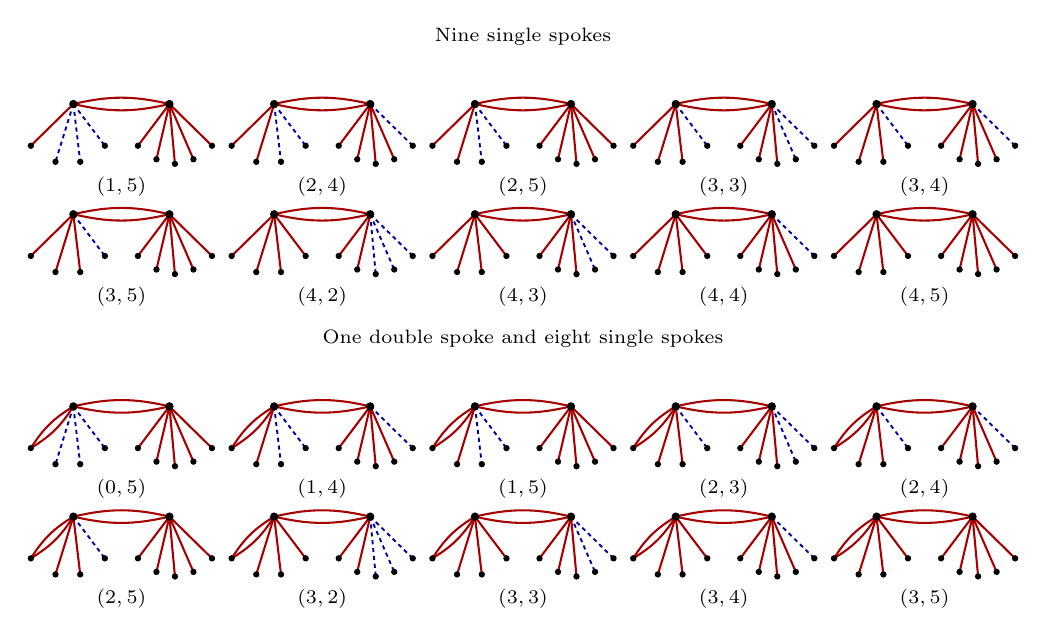
\begin{tikzpicture}[font=\scriptsize,
sc marked/.style={draw=red!65!black,line width=.75pt},
sc unmarked/.style={draw=blue!65!black,line width=.68pt,dash pattern=on 1.5pt off 1.35pt}]
\node[inner sep=0pt] at (0,0) {Nine single spokes};
\begin{scope}[shift={(-5.1,-0.89)}]
\coordinate (u) at (-0.61,0.03);
\coordinate (v) at (0.61,0.03);
\coordinate (u0) at (-1.15,-0.5);
\coordinate (u1) at (-0.837,-0.704);
\coordinate (u2) at (-0.523,-0.704);
\coordinate (u3) at (-0.21,-0.5);
\coordinate (v0) at (0.21,-0.5);
\coordinate (v1) at (0.445,-0.672);
\coordinate (v2) at (0.68,-0.73);
\coordinate (v3) at (0.915,-0.672);
\coordinate (v4) at (1.15,-0.5);
\draw[sc marked] (u) to[bend left=13] (v);
\draw[sc marked] (u) to[bend right=13] (v);
\draw[sc marked] (u) -- (u0);
\draw[sc unmarked] (u) -- (u1);
\draw[sc unmarked] (u) -- (u2);
\draw[sc unmarked] (u) -- (u3);
\draw[sc marked] (v) -- (v0);
\draw[sc marked] (v) -- (v1);
\draw[sc marked] (v) -- (v2);
\draw[sc marked] (v) -- (v3);
\draw[sc marked] (v) -- (v4);
\fill (u) circle[radius=1.5pt];
\fill (v) circle[radius=1.5pt];
\fill (u0) circle[radius=1.15pt];
\fill (u1) circle[radius=1.15pt];
\fill (u2) circle[radius=1.15pt];
\fill (u3) circle[radius=1.15pt];
\fill (v0) circle[radius=1.15pt];
\fill (v1) circle[radius=1.15pt];
\fill (v2) circle[radius=1.15pt];
\fill (v3) circle[radius=1.15pt];
\fill (v4) circle[radius=1.15pt];
\node[anchor=north,inner sep=1pt] at (0,-.85) {\((1,5)\)};
\end{scope}
\begin{scope}[shift={(-2.55,-0.89)}]
\coordinate (u) at (-0.61,0.03);
\coordinate (v) at (0.61,0.03);
\coordinate (u0) at (-1.15,-0.5);
\coordinate (u1) at (-0.837,-0.704);
\coordinate (u2) at (-0.523,-0.704);
\coordinate (u3) at (-0.21,-0.5);
\coordinate (v0) at (0.21,-0.5);
\coordinate (v1) at (0.445,-0.672);
\coordinate (v2) at (0.68,-0.73);
\coordinate (v3) at (0.915,-0.672);
\coordinate (v4) at (1.15,-0.5);
\draw[sc marked] (u) to[bend left=13] (v);
\draw[sc marked] (u) to[bend right=13] (v);
\draw[sc marked] (u) -- (u0);
\draw[sc marked] (u) -- (u1);
\draw[sc unmarked] (u) -- (u2);
\draw[sc unmarked] (u) -- (u3);
\draw[sc marked] (v) -- (v0);
\draw[sc marked] (v) -- (v1);
\draw[sc marked] (v) -- (v2);
\draw[sc marked] (v) -- (v3);
\draw[sc unmarked] (v) -- (v4);
\fill (u) circle[radius=1.5pt];
\fill (v) circle[radius=1.5pt];
\fill (u0) circle[radius=1.15pt];
\fill (u1) circle[radius=1.15pt];
\fill (u2) circle[radius=1.15pt];
\fill (u3) circle[radius=1.15pt];
\fill (v0) circle[radius=1.15pt];
\fill (v1) circle[radius=1.15pt];
\fill (v2) circle[radius=1.15pt];
\fill (v3) circle[radius=1.15pt];
\fill (v4) circle[radius=1.15pt];
\node[anchor=north,inner sep=1pt] at (0,-.85) {\((2,4)\)};
\end{scope}
\begin{scope}[shift={(0,-0.89)}]
\coordinate (u) at (-0.61,0.03);
\coordinate (v) at (0.61,0.03);
\coordinate (u0) at (-1.15,-0.5);
\coordinate (u1) at (-0.837,-0.704);
\coordinate (u2) at (-0.523,-0.704);
\coordinate (u3) at (-0.21,-0.5);
\coordinate (v0) at (0.21,-0.5);
\coordinate (v1) at (0.445,-0.672);
\coordinate (v2) at (0.68,-0.73);
\coordinate (v3) at (0.915,-0.672);
\coordinate (v4) at (1.15,-0.5);
\draw[sc marked] (u) to[bend left=13] (v);
\draw[sc marked] (u) to[bend right=13] (v);
\draw[sc marked] (u) -- (u0);
\draw[sc marked] (u) -- (u1);
\draw[sc unmarked] (u) -- (u2);
\draw[sc unmarked] (u) -- (u3);
\draw[sc marked] (v) -- (v0);
\draw[sc marked] (v) -- (v1);
\draw[sc marked] (v) -- (v2);
\draw[sc marked] (v) -- (v3);
\draw[sc marked] (v) -- (v4);
\fill (u) circle[radius=1.5pt];
\fill (v) circle[radius=1.5pt];
\fill (u0) circle[radius=1.15pt];
\fill (u1) circle[radius=1.15pt];
\fill (u2) circle[radius=1.15pt];
\fill (u3) circle[radius=1.15pt];
\fill (v0) circle[radius=1.15pt];
\fill (v1) circle[radius=1.15pt];
\fill (v2) circle[radius=1.15pt];
\fill (v3) circle[radius=1.15pt];
\fill (v4) circle[radius=1.15pt];
\node[anchor=north,inner sep=1pt] at (0,-.85) {\((2,5)\)};
\end{scope}
\begin{scope}[shift={(2.55,-0.89)}]
\coordinate (u) at (-0.61,0.03);
\coordinate (v) at (0.61,0.03);
\coordinate (u0) at (-1.15,-0.5);
\coordinate (u1) at (-0.837,-0.704);
\coordinate (u2) at (-0.523,-0.704);
\coordinate (u3) at (-0.21,-0.5);
\coordinate (v0) at (0.21,-0.5);
\coordinate (v1) at (0.445,-0.672);
\coordinate (v2) at (0.68,-0.73);
\coordinate (v3) at (0.915,-0.672);
\coordinate (v4) at (1.15,-0.5);
\draw[sc marked] (u) to[bend left=13] (v);
\draw[sc marked] (u) to[bend right=13] (v);
\draw[sc marked] (u) -- (u0);
\draw[sc marked] (u) -- (u1);
\draw[sc marked] (u) -- (u2);
\draw[sc unmarked] (u) -- (u3);
\draw[sc marked] (v) -- (v0);
\draw[sc marked] (v) -- (v1);
\draw[sc marked] (v) -- (v2);
\draw[sc unmarked] (v) -- (v3);
\draw[sc unmarked] (v) -- (v4);
\fill (u) circle[radius=1.5pt];
\fill (v) circle[radius=1.5pt];
\fill (u0) circle[radius=1.15pt];
\fill (u1) circle[radius=1.15pt];
\fill (u2) circle[radius=1.15pt];
\fill (u3) circle[radius=1.15pt];
\fill (v0) circle[radius=1.15pt];
\fill (v1) circle[radius=1.15pt];
\fill (v2) circle[radius=1.15pt];
\fill (v3) circle[radius=1.15pt];
\fill (v4) circle[radius=1.15pt];
\node[anchor=north,inner sep=1pt] at (0,-.85) {\((3,3)\)};
\end{scope}
\begin{scope}[shift={(5.1,-0.89)}]
\coordinate (u) at (-0.61,0.03);
\coordinate (v) at (0.61,0.03);
\coordinate (u0) at (-1.15,-0.5);
\coordinate (u1) at (-0.837,-0.704);
\coordinate (u2) at (-0.523,-0.704);
\coordinate (u3) at (-0.21,-0.5);
\coordinate (v0) at (0.21,-0.5);
\coordinate (v1) at (0.445,-0.672);
\coordinate (v2) at (0.68,-0.73);
\coordinate (v3) at (0.915,-0.672);
\coordinate (v4) at (1.15,-0.5);
\draw[sc marked] (u) to[bend left=13] (v);
\draw[sc marked] (u) to[bend right=13] (v);
\draw[sc marked] (u) -- (u0);
\draw[sc marked] (u) -- (u1);
\draw[sc marked] (u) -- (u2);
\draw[sc unmarked] (u) -- (u3);
\draw[sc marked] (v) -- (v0);
\draw[sc marked] (v) -- (v1);
\draw[sc marked] (v) -- (v2);
\draw[sc marked] (v) -- (v3);
\draw[sc unmarked] (v) -- (v4);
\fill (u) circle[radius=1.5pt];
\fill (v) circle[radius=1.5pt];
\fill (u0) circle[radius=1.15pt];
\fill (u1) circle[radius=1.15pt];
\fill (u2) circle[radius=1.15pt];
\fill (u3) circle[radius=1.15pt];
\fill (v0) circle[radius=1.15pt];
\fill (v1) circle[radius=1.15pt];
\fill (v2) circle[radius=1.15pt];
\fill (v3) circle[radius=1.15pt];
\fill (v4) circle[radius=1.15pt];
\node[anchor=north,inner sep=1pt] at (0,-.85) {\((3,4)\)};
\end{scope}
\begin{scope}[shift={(-5.1,-2.29)}]
\coordinate (u) at (-0.61,0.03);
\coordinate (v) at (0.61,0.03);
\coordinate (u0) at (-1.15,-0.5);
\coordinate (u1) at (-0.837,-0.704);
\coordinate (u2) at (-0.523,-0.704);
\coordinate (u3) at (-0.21,-0.5);
\coordinate (v0) at (0.21,-0.5);
\coordinate (v1) at (0.445,-0.672);
\coordinate (v2) at (0.68,-0.73);
\coordinate (v3) at (0.915,-0.672);
\coordinate (v4) at (1.15,-0.5);
\draw[sc marked] (u) to[bend left=13] (v);
\draw[sc marked] (u) to[bend right=13] (v);
\draw[sc marked] (u) -- (u0);
\draw[sc marked] (u) -- (u1);
\draw[sc marked] (u) -- (u2);
\draw[sc unmarked] (u) -- (u3);
\draw[sc marked] (v) -- (v0);
\draw[sc marked] (v) -- (v1);
\draw[sc marked] (v) -- (v2);
\draw[sc marked] (v) -- (v3);
\draw[sc marked] (v) -- (v4);
\fill (u) circle[radius=1.5pt];
\fill (v) circle[radius=1.5pt];
\fill (u0) circle[radius=1.15pt];
\fill (u1) circle[radius=1.15pt];
\fill (u2) circle[radius=1.15pt];
\fill (u3) circle[radius=1.15pt];
\fill (v0) circle[radius=1.15pt];
\fill (v1) circle[radius=1.15pt];
\fill (v2) circle[radius=1.15pt];
\fill (v3) circle[radius=1.15pt];
\fill (v4) circle[radius=1.15pt];
\node[anchor=north,inner sep=1pt] at (0,-.85) {\((3,5)\)};
\end{scope}
\begin{scope}[shift={(-2.55,-2.29)}]
\coordinate (u) at (-0.61,0.03);
\coordinate (v) at (0.61,0.03);
\coordinate (u0) at (-1.15,-0.5);
\coordinate (u1) at (-0.837,-0.704);
\coordinate (u2) at (-0.523,-0.704);
\coordinate (u3) at (-0.21,-0.5);
\coordinate (v0) at (0.21,-0.5);
\coordinate (v1) at (0.445,-0.672);
\coordinate (v2) at (0.68,-0.73);
\coordinate (v3) at (0.915,-0.672);
\coordinate (v4) at (1.15,-0.5);
\draw[sc marked] (u) to[bend left=13] (v);
\draw[sc marked] (u) to[bend right=13] (v);
\draw[sc marked] (u) -- (u0);
\draw[sc marked] (u) -- (u1);
\draw[sc marked] (u) -- (u2);
\draw[sc marked] (u) -- (u3);
\draw[sc marked] (v) -- (v0);
\draw[sc marked] (v) -- (v1);
\draw[sc unmarked] (v) -- (v2);
\draw[sc unmarked] (v) -- (v3);
\draw[sc unmarked] (v) -- (v4);
\fill (u) circle[radius=1.5pt];
\fill (v) circle[radius=1.5pt];
\fill (u0) circle[radius=1.15pt];
\fill (u1) circle[radius=1.15pt];
\fill (u2) circle[radius=1.15pt];
\fill (u3) circle[radius=1.15pt];
\fill (v0) circle[radius=1.15pt];
\fill (v1) circle[radius=1.15pt];
\fill (v2) circle[radius=1.15pt];
\fill (v3) circle[radius=1.15pt];
\fill (v4) circle[radius=1.15pt];
\node[anchor=north,inner sep=1pt] at (0,-.85) {\((4,2)\)};
\end{scope}
\begin{scope}[shift={(0,-2.29)}]
\coordinate (u) at (-0.61,0.03);
\coordinate (v) at (0.61,0.03);
\coordinate (u0) at (-1.15,-0.5);
\coordinate (u1) at (-0.837,-0.704);
\coordinate (u2) at (-0.523,-0.704);
\coordinate (u3) at (-0.21,-0.5);
\coordinate (v0) at (0.21,-0.5);
\coordinate (v1) at (0.445,-0.672);
\coordinate (v2) at (0.68,-0.73);
\coordinate (v3) at (0.915,-0.672);
\coordinate (v4) at (1.15,-0.5);
\draw[sc marked] (u) to[bend left=13] (v);
\draw[sc marked] (u) to[bend right=13] (v);
\draw[sc marked] (u) -- (u0);
\draw[sc marked] (u) -- (u1);
\draw[sc marked] (u) -- (u2);
\draw[sc marked] (u) -- (u3);
\draw[sc marked] (v) -- (v0);
\draw[sc marked] (v) -- (v1);
\draw[sc marked] (v) -- (v2);
\draw[sc unmarked] (v) -- (v3);
\draw[sc unmarked] (v) -- (v4);
\fill (u) circle[radius=1.5pt];
\fill (v) circle[radius=1.5pt];
\fill (u0) circle[radius=1.15pt];
\fill (u1) circle[radius=1.15pt];
\fill (u2) circle[radius=1.15pt];
\fill (u3) circle[radius=1.15pt];
\fill (v0) circle[radius=1.15pt];
\fill (v1) circle[radius=1.15pt];
\fill (v2) circle[radius=1.15pt];
\fill (v3) circle[radius=1.15pt];
\fill (v4) circle[radius=1.15pt];
\node[anchor=north,inner sep=1pt] at (0,-.85) {\((4,3)\)};
\end{scope}
\begin{scope}[shift={(2.55,-2.29)}]
\coordinate (u) at (-0.61,0.03);
\coordinate (v) at (0.61,0.03);
\coordinate (u0) at (-1.15,-0.5);
\coordinate (u1) at (-0.837,-0.704);
\coordinate (u2) at (-0.523,-0.704);
\coordinate (u3) at (-0.21,-0.5);
\coordinate (v0) at (0.21,-0.5);
\coordinate (v1) at (0.445,-0.672);
\coordinate (v2) at (0.68,-0.73);
\coordinate (v3) at (0.915,-0.672);
\coordinate (v4) at (1.15,-0.5);
\draw[sc marked] (u) to[bend left=13] (v);
\draw[sc marked] (u) to[bend right=13] (v);
\draw[sc marked] (u) -- (u0);
\draw[sc marked] (u) -- (u1);
\draw[sc marked] (u) -- (u2);
\draw[sc marked] (u) -- (u3);
\draw[sc marked] (v) -- (v0);
\draw[sc marked] (v) -- (v1);
\draw[sc marked] (v) -- (v2);
\draw[sc marked] (v) -- (v3);
\draw[sc unmarked] (v) -- (v4);
\fill (u) circle[radius=1.5pt];
\fill (v) circle[radius=1.5pt];
\fill (u0) circle[radius=1.15pt];
\fill (u1) circle[radius=1.15pt];
\fill (u2) circle[radius=1.15pt];
\fill (u3) circle[radius=1.15pt];
\fill (v0) circle[radius=1.15pt];
\fill (v1) circle[radius=1.15pt];
\fill (v2) circle[radius=1.15pt];
\fill (v3) circle[radius=1.15pt];
\fill (v4) circle[radius=1.15pt];
\node[anchor=north,inner sep=1pt] at (0,-.85) {\((4,4)\)};
\end{scope}
\begin{scope}[shift={(5.1,-2.29)}]
\coordinate (u) at (-0.61,0.03);
\coordinate (v) at (0.61,0.03);
\coordinate (u0) at (-1.15,-0.5);
\coordinate (u1) at (-0.837,-0.704);
\coordinate (u2) at (-0.523,-0.704);
\coordinate (u3) at (-0.21,-0.5);
\coordinate (v0) at (0.21,-0.5);
\coordinate (v1) at (0.445,-0.672);
\coordinate (v2) at (0.68,-0.73);
\coordinate (v3) at (0.915,-0.672);
\coordinate (v4) at (1.15,-0.5);
\draw[sc marked] (u) to[bend left=13] (v);
\draw[sc marked] (u) to[bend right=13] (v);
\draw[sc marked] (u) -- (u0);
\draw[sc marked] (u) -- (u1);
\draw[sc marked] (u) -- (u2);
\draw[sc marked] (u) -- (u3);
\draw[sc marked] (v) -- (v0);
\draw[sc marked] (v) -- (v1);
\draw[sc marked] (v) -- (v2);
\draw[sc marked] (v) -- (v3);
\draw[sc marked] (v) -- (v4);
\fill (u) circle[radius=1.5pt];
\fill (v) circle[radius=1.5pt];
\fill (u0) circle[radius=1.15pt];
\fill (u1) circle[radius=1.15pt];
\fill (u2) circle[radius=1.15pt];
\fill (u3) circle[radius=1.15pt];
\fill (v0) circle[radius=1.15pt];
\fill (v1) circle[radius=1.15pt];
\fill (v2) circle[radius=1.15pt];
\fill (v3) circle[radius=1.15pt];
\fill (v4) circle[radius=1.15pt];
\node[anchor=north,inner sep=1pt] at (0,-.85) {\((4,5)\)};
\end{scope}
\node[inner sep=0pt] at (0,-3.84) {One double spoke and eight single spokes};
\begin{scope}[shift={(-5.1,-4.73)}]
\coordinate (u) at (-0.61,0.03);
\coordinate (v) at (0.61,0.03);
\coordinate (u0) at (-1.15,-0.5);
\coordinate (u1) at (-0.837,-0.704);
\coordinate (u2) at (-0.523,-0.704);
\coordinate (u3) at (-0.21,-0.5);
\coordinate (v0) at (0.21,-0.5);
\coordinate (v1) at (0.445,-0.672);
\coordinate (v2) at (0.68,-0.73);
\coordinate (v3) at (0.915,-0.672);
\coordinate (v4) at (1.15,-0.5);
\draw[sc marked] (u) to[bend left=13] (v);
\draw[sc marked] (u) to[bend right=13] (v);
\draw[sc marked] (u) to[bend left=13] (u0);
\draw[sc marked] (u) to[bend right=13] (u0);
\draw[sc unmarked] (u) -- (u1);
\draw[sc unmarked] (u) -- (u2);
\draw[sc unmarked] (u) -- (u3);
\draw[sc marked] (v) -- (v0);
\draw[sc marked] (v) -- (v1);
\draw[sc marked] (v) -- (v2);
\draw[sc marked] (v) -- (v3);
\draw[sc marked] (v) -- (v4);
\fill (u) circle[radius=1.5pt];
\fill (v) circle[radius=1.5pt];
\fill (u0) circle[radius=1.15pt];
\fill (u1) circle[radius=1.15pt];
\fill (u2) circle[radius=1.15pt];
\fill (u3) circle[radius=1.15pt];
\fill (v0) circle[radius=1.15pt];
\fill (v1) circle[radius=1.15pt];
\fill (v2) circle[radius=1.15pt];
\fill (v3) circle[radius=1.15pt];
\fill (v4) circle[radius=1.15pt];
\node[anchor=north,inner sep=1pt] at (0,-.85) {\((0,5)\)};
\end{scope}
\begin{scope}[shift={(-2.55,-4.73)}]
\coordinate (u) at (-0.61,0.03);
\coordinate (v) at (0.61,0.03);
\coordinate (u0) at (-1.15,-0.5);
\coordinate (u1) at (-0.837,-0.704);
\coordinate (u2) at (-0.523,-0.704);
\coordinate (u3) at (-0.21,-0.5);
\coordinate (v0) at (0.21,-0.5);
\coordinate (v1) at (0.445,-0.672);
\coordinate (v2) at (0.68,-0.73);
\coordinate (v3) at (0.915,-0.672);
\coordinate (v4) at (1.15,-0.5);
\draw[sc marked] (u) to[bend left=13] (v);
\draw[sc marked] (u) to[bend right=13] (v);
\draw[sc marked] (u) to[bend left=13] (u0);
\draw[sc marked] (u) to[bend right=13] (u0);
\draw[sc marked] (u) -- (u1);
\draw[sc unmarked] (u) -- (u2);
\draw[sc unmarked] (u) -- (u3);
\draw[sc marked] (v) -- (v0);
\draw[sc marked] (v) -- (v1);
\draw[sc marked] (v) -- (v2);
\draw[sc marked] (v) -- (v3);
\draw[sc unmarked] (v) -- (v4);
\fill (u) circle[radius=1.5pt];
\fill (v) circle[radius=1.5pt];
\fill (u0) circle[radius=1.15pt];
\fill (u1) circle[radius=1.15pt];
\fill (u2) circle[radius=1.15pt];
\fill (u3) circle[radius=1.15pt];
\fill (v0) circle[radius=1.15pt];
\fill (v1) circle[radius=1.15pt];
\fill (v2) circle[radius=1.15pt];
\fill (v3) circle[radius=1.15pt];
\fill (v4) circle[radius=1.15pt];
\node[anchor=north,inner sep=1pt] at (0,-.85) {\((1,4)\)};
\end{scope}
\begin{scope}[shift={(0,-4.73)}]
\coordinate (u) at (-0.61,0.03);
\coordinate (v) at (0.61,0.03);
\coordinate (u0) at (-1.15,-0.5);
\coordinate (u1) at (-0.837,-0.704);
\coordinate (u2) at (-0.523,-0.704);
\coordinate (u3) at (-0.21,-0.5);
\coordinate (v0) at (0.21,-0.5);
\coordinate (v1) at (0.445,-0.672);
\coordinate (v2) at (0.68,-0.73);
\coordinate (v3) at (0.915,-0.672);
\coordinate (v4) at (1.15,-0.5);
\draw[sc marked] (u) to[bend left=13] (v);
\draw[sc marked] (u) to[bend right=13] (v);
\draw[sc marked] (u) to[bend left=13] (u0);
\draw[sc marked] (u) to[bend right=13] (u0);
\draw[sc marked] (u) -- (u1);
\draw[sc unmarked] (u) -- (u2);
\draw[sc unmarked] (u) -- (u3);
\draw[sc marked] (v) -- (v0);
\draw[sc marked] (v) -- (v1);
\draw[sc marked] (v) -- (v2);
\draw[sc marked] (v) -- (v3);
\draw[sc marked] (v) -- (v4);
\fill (u) circle[radius=1.5pt];
\fill (v) circle[radius=1.5pt];
\fill (u0) circle[radius=1.15pt];
\fill (u1) circle[radius=1.15pt];
\fill (u2) circle[radius=1.15pt];
\fill (u3) circle[radius=1.15pt];
\fill (v0) circle[radius=1.15pt];
\fill (v1) circle[radius=1.15pt];
\fill (v2) circle[radius=1.15pt];
\fill (v3) circle[radius=1.15pt];
\fill (v4) circle[radius=1.15pt];
\node[anchor=north,inner sep=1pt] at (0,-.85) {\((1,5)\)};
\end{scope}
\begin{scope}[shift={(2.55,-4.73)}]
\coordinate (u) at (-0.61,0.03);
\coordinate (v) at (0.61,0.03);
\coordinate (u0) at (-1.15,-0.5);
\coordinate (u1) at (-0.837,-0.704);
\coordinate (u2) at (-0.523,-0.704);
\coordinate (u3) at (-0.21,-0.5);
\coordinate (v0) at (0.21,-0.5);
\coordinate (v1) at (0.445,-0.672);
\coordinate (v2) at (0.68,-0.73);
\coordinate (v3) at (0.915,-0.672);
\coordinate (v4) at (1.15,-0.5);
\draw[sc marked] (u) to[bend left=13] (v);
\draw[sc marked] (u) to[bend right=13] (v);
\draw[sc marked] (u) to[bend left=13] (u0);
\draw[sc marked] (u) to[bend right=13] (u0);
\draw[sc marked] (u) -- (u1);
\draw[sc marked] (u) -- (u2);
\draw[sc unmarked] (u) -- (u3);
\draw[sc marked] (v) -- (v0);
\draw[sc marked] (v) -- (v1);
\draw[sc marked] (v) -- (v2);
\draw[sc unmarked] (v) -- (v3);
\draw[sc unmarked] (v) -- (v4);
\fill (u) circle[radius=1.5pt];
\fill (v) circle[radius=1.5pt];
\fill (u0) circle[radius=1.15pt];
\fill (u1) circle[radius=1.15pt];
\fill (u2) circle[radius=1.15pt];
\fill (u3) circle[radius=1.15pt];
\fill (v0) circle[radius=1.15pt];
\fill (v1) circle[radius=1.15pt];
\fill (v2) circle[radius=1.15pt];
\fill (v3) circle[radius=1.15pt];
\fill (v4) circle[radius=1.15pt];
\node[anchor=north,inner sep=1pt] at (0,-.85) {\((2,3)\)};
\end{scope}
\begin{scope}[shift={(5.1,-4.73)}]
\coordinate (u) at (-0.61,0.03);
\coordinate (v) at (0.61,0.03);
\coordinate (u0) at (-1.15,-0.5);
\coordinate (u1) at (-0.837,-0.704);
\coordinate (u2) at (-0.523,-0.704);
\coordinate (u3) at (-0.21,-0.5);
\coordinate (v0) at (0.21,-0.5);
\coordinate (v1) at (0.445,-0.672);
\coordinate (v2) at (0.68,-0.73);
\coordinate (v3) at (0.915,-0.672);
\coordinate (v4) at (1.15,-0.5);
\draw[sc marked] (u) to[bend left=13] (v);
\draw[sc marked] (u) to[bend right=13] (v);
\draw[sc marked] (u) to[bend left=13] (u0);
\draw[sc marked] (u) to[bend right=13] (u0);
\draw[sc marked] (u) -- (u1);
\draw[sc marked] (u) -- (u2);
\draw[sc unmarked] (u) -- (u3);
\draw[sc marked] (v) -- (v0);
\draw[sc marked] (v) -- (v1);
\draw[sc marked] (v) -- (v2);
\draw[sc marked] (v) -- (v3);
\draw[sc unmarked] (v) -- (v4);
\fill (u) circle[radius=1.5pt];
\fill (v) circle[radius=1.5pt];
\fill (u0) circle[radius=1.15pt];
\fill (u1) circle[radius=1.15pt];
\fill (u2) circle[radius=1.15pt];
\fill (u3) circle[radius=1.15pt];
\fill (v0) circle[radius=1.15pt];
\fill (v1) circle[radius=1.15pt];
\fill (v2) circle[radius=1.15pt];
\fill (v3) circle[radius=1.15pt];
\fill (v4) circle[radius=1.15pt];
\node[anchor=north,inner sep=1pt] at (0,-.85) {\((2,4)\)};
\end{scope}
\begin{scope}[shift={(-5.1,-6.13)}]
\coordinate (u) at (-0.61,0.03);
\coordinate (v) at (0.61,0.03);
\coordinate (u0) at (-1.15,-0.5);
\coordinate (u1) at (-0.837,-0.704);
\coordinate (u2) at (-0.523,-0.704);
\coordinate (u3) at (-0.21,-0.5);
\coordinate (v0) at (0.21,-0.5);
\coordinate (v1) at (0.445,-0.672);
\coordinate (v2) at (0.68,-0.73);
\coordinate (v3) at (0.915,-0.672);
\coordinate (v4) at (1.15,-0.5);
\draw[sc marked] (u) to[bend left=13] (v);
\draw[sc marked] (u) to[bend right=13] (v);
\draw[sc marked] (u) to[bend left=13] (u0);
\draw[sc marked] (u) to[bend right=13] (u0);
\draw[sc marked] (u) -- (u1);
\draw[sc marked] (u) -- (u2);
\draw[sc unmarked] (u) -- (u3);
\draw[sc marked] (v) -- (v0);
\draw[sc marked] (v) -- (v1);
\draw[sc marked] (v) -- (v2);
\draw[sc marked] (v) -- (v3);
\draw[sc marked] (v) -- (v4);
\fill (u) circle[radius=1.5pt];
\fill (v) circle[radius=1.5pt];
\fill (u0) circle[radius=1.15pt];
\fill (u1) circle[radius=1.15pt];
\fill (u2) circle[radius=1.15pt];
\fill (u3) circle[radius=1.15pt];
\fill (v0) circle[radius=1.15pt];
\fill (v1) circle[radius=1.15pt];
\fill (v2) circle[radius=1.15pt];
\fill (v3) circle[radius=1.15pt];
\fill (v4) circle[radius=1.15pt];
\node[anchor=north,inner sep=1pt] at (0,-.85) {\((2,5)\)};
\end{scope}
\begin{scope}[shift={(-2.55,-6.13)}]
\coordinate (u) at (-0.61,0.03);
\coordinate (v) at (0.61,0.03);
\coordinate (u0) at (-1.15,-0.5);
\coordinate (u1) at (-0.837,-0.704);
\coordinate (u2) at (-0.523,-0.704);
\coordinate (u3) at (-0.21,-0.5);
\coordinate (v0) at (0.21,-0.5);
\coordinate (v1) at (0.445,-0.672);
\coordinate (v2) at (0.68,-0.73);
\coordinate (v3) at (0.915,-0.672);
\coordinate (v4) at (1.15,-0.5);
\draw[sc marked] (u) to[bend left=13] (v);
\draw[sc marked] (u) to[bend right=13] (v);
\draw[sc marked] (u) to[bend left=13] (u0);
\draw[sc marked] (u) to[bend right=13] (u0);
\draw[sc marked] (u) -- (u1);
\draw[sc marked] (u) -- (u2);
\draw[sc marked] (u) -- (u3);
\draw[sc marked] (v) -- (v0);
\draw[sc marked] (v) -- (v1);
\draw[sc unmarked] (v) -- (v2);
\draw[sc unmarked] (v) -- (v3);
\draw[sc unmarked] (v) -- (v4);
\fill (u) circle[radius=1.5pt];
\fill (v) circle[radius=1.5pt];
\fill (u0) circle[radius=1.15pt];
\fill (u1) circle[radius=1.15pt];
\fill (u2) circle[radius=1.15pt];
\fill (u3) circle[radius=1.15pt];
\fill (v0) circle[radius=1.15pt];
\fill (v1) circle[radius=1.15pt];
\fill (v2) circle[radius=1.15pt];
\fill (v3) circle[radius=1.15pt];
\fill (v4) circle[radius=1.15pt];
\node[anchor=north,inner sep=1pt] at (0,-.85) {\((3,2)\)};
\end{scope}
\begin{scope}[shift={(0,-6.13)}]
\coordinate (u) at (-0.61,0.03);
\coordinate (v) at (0.61,0.03);
\coordinate (u0) at (-1.15,-0.5);
\coordinate (u1) at (-0.837,-0.704);
\coordinate (u2) at (-0.523,-0.704);
\coordinate (u3) at (-0.21,-0.5);
\coordinate (v0) at (0.21,-0.5);
\coordinate (v1) at (0.445,-0.672);
\coordinate (v2) at (0.68,-0.73);
\coordinate (v3) at (0.915,-0.672);
\coordinate (v4) at (1.15,-0.5);
\draw[sc marked] (u) to[bend left=13] (v);
\draw[sc marked] (u) to[bend right=13] (v);
\draw[sc marked] (u) to[bend left=13] (u0);
\draw[sc marked] (u) to[bend right=13] (u0);
\draw[sc marked] (u) -- (u1);
\draw[sc marked] (u) -- (u2);
\draw[sc marked] (u) -- (u3);
\draw[sc marked] (v) -- (v0);
\draw[sc marked] (v) -- (v1);
\draw[sc marked] (v) -- (v2);
\draw[sc unmarked] (v) -- (v3);
\draw[sc unmarked] (v) -- (v4);
\fill (u) circle[radius=1.5pt];
\fill (v) circle[radius=1.5pt];
\fill (u0) circle[radius=1.15pt];
\fill (u1) circle[radius=1.15pt];
\fill (u2) circle[radius=1.15pt];
\fill (u3) circle[radius=1.15pt];
\fill (v0) circle[radius=1.15pt];
\fill (v1) circle[radius=1.15pt];
\fill (v2) circle[radius=1.15pt];
\fill (v3) circle[radius=1.15pt];
\fill (v4) circle[radius=1.15pt];
\node[anchor=north,inner sep=1pt] at (0,-.85) {\((3,3)\)};
\end{scope}
\begin{scope}[shift={(2.55,-6.13)}]
\coordinate (u) at (-0.61,0.03);
\coordinate (v) at (0.61,0.03);
\coordinate (u0) at (-1.15,-0.5);
\coordinate (u1) at (-0.837,-0.704);
\coordinate (u2) at (-0.523,-0.704);
\coordinate (u3) at (-0.21,-0.5);
\coordinate (v0) at (0.21,-0.5);
\coordinate (v1) at (0.445,-0.672);
\coordinate (v2) at (0.68,-0.73);
\coordinate (v3) at (0.915,-0.672);
\coordinate (v4) at (1.15,-0.5);
\draw[sc marked] (u) to[bend left=13] (v);
\draw[sc marked] (u) to[bend right=13] (v);
\draw[sc marked] (u) to[bend left=13] (u0);
\draw[sc marked] (u) to[bend right=13] (u0);
\draw[sc marked] (u) -- (u1);
\draw[sc marked] (u) -- (u2);
\draw[sc marked] (u) -- (u3);
\draw[sc marked] (v) -- (v0);
\draw[sc marked] (v) -- (v1);
\draw[sc marked] (v) -- (v2);
\draw[sc marked] (v) -- (v3);
\draw[sc unmarked] (v) -- (v4);
\fill (u) circle[radius=1.5pt];
\fill (v) circle[radius=1.5pt];
\fill (u0) circle[radius=1.15pt];
\fill (u1) circle[radius=1.15pt];
\fill (u2) circle[radius=1.15pt];
\fill (u3) circle[radius=1.15pt];
\fill (v0) circle[radius=1.15pt];
\fill (v1) circle[radius=1.15pt];
\fill (v2) circle[radius=1.15pt];
\fill (v3) circle[radius=1.15pt];
\fill (v4) circle[radius=1.15pt];
\node[anchor=north,inner sep=1pt] at (0,-.85) {\((3,4)\)};
\end{scope}
\begin{scope}[shift={(5.1,-6.13)}]
\coordinate (u) at (-0.61,0.03);
\coordinate (v) at (0.61,0.03);
\coordinate (u0) at (-1.15,-0.5);
\coordinate (u1) at (-0.837,-0.704);
\coordinate (u2) at (-0.523,-0.704);
\coordinate (u3) at (-0.21,-0.5);
\coordinate (v0) at (0.21,-0.5);
\coordinate (v1) at (0.445,-0.672);
\coordinate (v2) at (0.68,-0.73);
\coordinate (v3) at (0.915,-0.672);
\coordinate (v4) at (1.15,-0.5);
\draw[sc marked] (u) to[bend left=13] (v);
\draw[sc marked] (u) to[bend right=13] (v);
\draw[sc marked] (u) to[bend left=13] (u0);
\draw[sc marked] (u) to[bend right=13] (u0);
\draw[sc marked] (u) -- (u1);
\draw[sc marked] (u) -- (u2);
\draw[sc marked] (u) -- (u3);
\draw[sc marked] (v) -- (v0);
\draw[sc marked] (v) -- (v1);
\draw[sc marked] (v) -- (v2);
\draw[sc marked] (v) -- (v3);
\draw[sc marked] (v) -- (v4);
\fill (u) circle[radius=1.5pt];
\fill (v) circle[radius=1.5pt];
\fill (u0) circle[radius=1.15pt];
\fill (u1) circle[radius=1.15pt];
\fill (u2) circle[radius=1.15pt];
\fill (u3) circle[radius=1.15pt];
\fill (v0) circle[radius=1.15pt];
\fill (v1) circle[radius=1.15pt];
\fill (v2) circle[radius=1.15pt];
\fill (v3) circle[radius=1.15pt];
\fill (v4) circle[radius=1.15pt];
\node[anchor=north,inner sep=1pt] at (0,-.85) {\((3,5)\)};
\end{scope}
\end{tikzpicture}
\caption{The 20 degree-seven configurations with $q=9$ and disjoint root neighborhoods outside the root pair. Each label counts only the marked single spokes at the two roots.}
\label{fig:finite-seven-separate}
\end{figure}


If the roots share a neighbor outside $\{u,v\}$, the nine neighbors
require at least ten spokes. Thus all ten spokes are single and each
root has four neighbors that are nonadjacent to the other root.
The choices of marked spokes to those vertices and the
two spokes to the common neighbor give the fourteen configurations in
\textbf{Figure~\ref{fig:finite-seven-shared}}.

\begin{figure}[htbp]
\centering
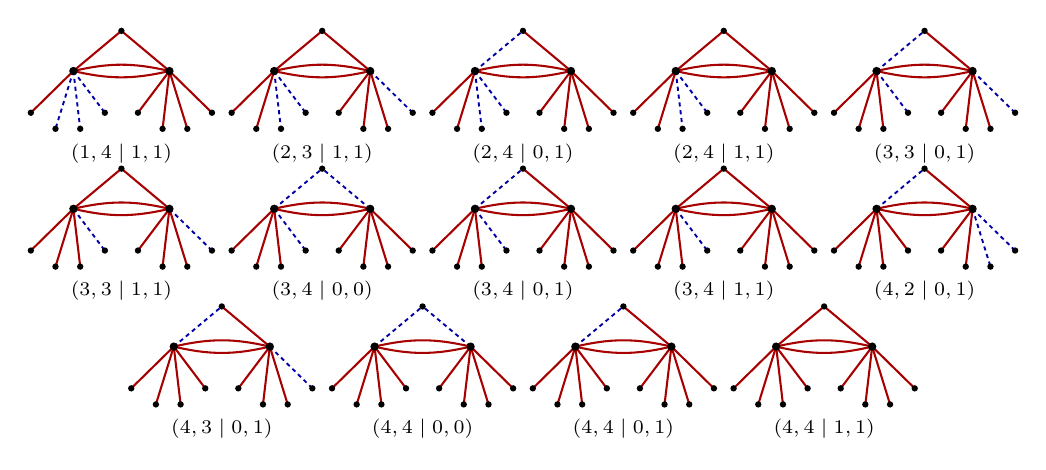
\begin{tikzpicture}[font=\scriptsize,
sc marked/.style={draw=red!65!black,line width=.75pt},
sc unmarked/.style={draw=blue!65!black,line width=.68pt,dash pattern=on 1.5pt off 1.35pt}]
\begin{scope}[shift={(-5.1,0)}]
\coordinate (u) at (-0.61,0.03);
\coordinate (v) at (0.61,0.03);
\coordinate (u0) at (-1.15,-0.5);
\coordinate (u1) at (-0.837,-0.704);
\coordinate (u2) at (-0.523,-0.704);
\coordinate (u3) at (-0.21,-0.5);
\coordinate (v0) at (0.21,-0.5);
\coordinate (v1) at (0.523,-0.704);
\coordinate (v2) at (0.837,-0.704);
\coordinate (v3) at (1.15,-0.5);
\coordinate (w) at (0,0.54);
\draw[sc marked] (u) to[bend left=13] (v);
\draw[sc marked] (u) to[bend right=13] (v);
\draw[sc marked] (u) -- (u0);
\draw[sc unmarked] (u) -- (u1);
\draw[sc unmarked] (u) -- (u2);
\draw[sc unmarked] (u) -- (u3);
\draw[sc marked] (v) -- (v0);
\draw[sc marked] (v) -- (v1);
\draw[sc marked] (v) -- (v2);
\draw[sc marked] (v) -- (v3);
\draw[sc marked] (u) -- (w);
\draw[sc marked] (v) -- (w);
\fill (u) circle[radius=1.5pt];
\fill (v) circle[radius=1.5pt];
\fill (u0) circle[radius=1.15pt];
\fill (u1) circle[radius=1.15pt];
\fill (u2) circle[radius=1.15pt];
\fill (u3) circle[radius=1.15pt];
\fill (v0) circle[radius=1.15pt];
\fill (v1) circle[radius=1.15pt];
\fill (v2) circle[radius=1.15pt];
\fill (v3) circle[radius=1.15pt];
\fill (w) circle[radius=1.15pt];
\node[anchor=north,inner sep=1pt] at (0,-.85) {\((1,4\mid 1,1)\)};
\end{scope}
\begin{scope}[shift={(-2.55,0)}]
\coordinate (u) at (-0.61,0.03);
\coordinate (v) at (0.61,0.03);
\coordinate (u0) at (-1.15,-0.5);
\coordinate (u1) at (-0.837,-0.704);
\coordinate (u2) at (-0.523,-0.704);
\coordinate (u3) at (-0.21,-0.5);
\coordinate (v0) at (0.21,-0.5);
\coordinate (v1) at (0.523,-0.704);
\coordinate (v2) at (0.837,-0.704);
\coordinate (v3) at (1.15,-0.5);
\coordinate (w) at (0,0.54);
\draw[sc marked] (u) to[bend left=13] (v);
\draw[sc marked] (u) to[bend right=13] (v);
\draw[sc marked] (u) -- (u0);
\draw[sc marked] (u) -- (u1);
\draw[sc unmarked] (u) -- (u2);
\draw[sc unmarked] (u) -- (u3);
\draw[sc marked] (v) -- (v0);
\draw[sc marked] (v) -- (v1);
\draw[sc marked] (v) -- (v2);
\draw[sc unmarked] (v) -- (v3);
\draw[sc marked] (u) -- (w);
\draw[sc marked] (v) -- (w);
\fill (u) circle[radius=1.5pt];
\fill (v) circle[radius=1.5pt];
\fill (u0) circle[radius=1.15pt];
\fill (u1) circle[radius=1.15pt];
\fill (u2) circle[radius=1.15pt];
\fill (u3) circle[radius=1.15pt];
\fill (v0) circle[radius=1.15pt];
\fill (v1) circle[radius=1.15pt];
\fill (v2) circle[radius=1.15pt];
\fill (v3) circle[radius=1.15pt];
\fill (w) circle[radius=1.15pt];
\node[anchor=north,inner sep=1pt] at (0,-.85) {\((2,3\mid 1,1)\)};
\end{scope}
\begin{scope}[shift={(0,0)}]
\coordinate (u) at (-0.61,0.03);
\coordinate (v) at (0.61,0.03);
\coordinate (u0) at (-1.15,-0.5);
\coordinate (u1) at (-0.837,-0.704);
\coordinate (u2) at (-0.523,-0.704);
\coordinate (u3) at (-0.21,-0.5);
\coordinate (v0) at (0.21,-0.5);
\coordinate (v1) at (0.523,-0.704);
\coordinate (v2) at (0.837,-0.704);
\coordinate (v3) at (1.15,-0.5);
\coordinate (w) at (0,0.54);
\draw[sc marked] (u) to[bend left=13] (v);
\draw[sc marked] (u) to[bend right=13] (v);
\draw[sc marked] (u) -- (u0);
\draw[sc marked] (u) -- (u1);
\draw[sc unmarked] (u) -- (u2);
\draw[sc unmarked] (u) -- (u3);
\draw[sc marked] (v) -- (v0);
\draw[sc marked] (v) -- (v1);
\draw[sc marked] (v) -- (v2);
\draw[sc marked] (v) -- (v3);
\draw[sc unmarked] (u) -- (w);
\draw[sc marked] (v) -- (w);
\fill (u) circle[radius=1.5pt];
\fill (v) circle[radius=1.5pt];
\fill (u0) circle[radius=1.15pt];
\fill (u1) circle[radius=1.15pt];
\fill (u2) circle[radius=1.15pt];
\fill (u3) circle[radius=1.15pt];
\fill (v0) circle[radius=1.15pt];
\fill (v1) circle[radius=1.15pt];
\fill (v2) circle[radius=1.15pt];
\fill (v3) circle[radius=1.15pt];
\fill (w) circle[radius=1.15pt];
\node[anchor=north,inner sep=1pt] at (0,-.85) {\((2,4\mid 0,1)\)};
\end{scope}
\begin{scope}[shift={(2.55,0)}]
\coordinate (u) at (-0.61,0.03);
\coordinate (v) at (0.61,0.03);
\coordinate (u0) at (-1.15,-0.5);
\coordinate (u1) at (-0.837,-0.704);
\coordinate (u2) at (-0.523,-0.704);
\coordinate (u3) at (-0.21,-0.5);
\coordinate (v0) at (0.21,-0.5);
\coordinate (v1) at (0.523,-0.704);
\coordinate (v2) at (0.837,-0.704);
\coordinate (v3) at (1.15,-0.5);
\coordinate (w) at (0,0.54);
\draw[sc marked] (u) to[bend left=13] (v);
\draw[sc marked] (u) to[bend right=13] (v);
\draw[sc marked] (u) -- (u0);
\draw[sc marked] (u) -- (u1);
\draw[sc unmarked] (u) -- (u2);
\draw[sc unmarked] (u) -- (u3);
\draw[sc marked] (v) -- (v0);
\draw[sc marked] (v) -- (v1);
\draw[sc marked] (v) -- (v2);
\draw[sc marked] (v) -- (v3);
\draw[sc marked] (u) -- (w);
\draw[sc marked] (v) -- (w);
\fill (u) circle[radius=1.5pt];
\fill (v) circle[radius=1.5pt];
\fill (u0) circle[radius=1.15pt];
\fill (u1) circle[radius=1.15pt];
\fill (u2) circle[radius=1.15pt];
\fill (u3) circle[radius=1.15pt];
\fill (v0) circle[radius=1.15pt];
\fill (v1) circle[radius=1.15pt];
\fill (v2) circle[radius=1.15pt];
\fill (v3) circle[radius=1.15pt];
\fill (w) circle[radius=1.15pt];
\node[anchor=north,inner sep=1pt] at (0,-.85) {\((2,4\mid 1,1)\)};
\end{scope}
\begin{scope}[shift={(5.1,0)}]
\coordinate (u) at (-0.61,0.03);
\coordinate (v) at (0.61,0.03);
\coordinate (u0) at (-1.15,-0.5);
\coordinate (u1) at (-0.837,-0.704);
\coordinate (u2) at (-0.523,-0.704);
\coordinate (u3) at (-0.21,-0.5);
\coordinate (v0) at (0.21,-0.5);
\coordinate (v1) at (0.523,-0.704);
\coordinate (v2) at (0.837,-0.704);
\coordinate (v3) at (1.15,-0.5);
\coordinate (w) at (0,0.54);
\draw[sc marked] (u) to[bend left=13] (v);
\draw[sc marked] (u) to[bend right=13] (v);
\draw[sc marked] (u) -- (u0);
\draw[sc marked] (u) -- (u1);
\draw[sc marked] (u) -- (u2);
\draw[sc unmarked] (u) -- (u3);
\draw[sc marked] (v) -- (v0);
\draw[sc marked] (v) -- (v1);
\draw[sc marked] (v) -- (v2);
\draw[sc unmarked] (v) -- (v3);
\draw[sc unmarked] (u) -- (w);
\draw[sc marked] (v) -- (w);
\fill (u) circle[radius=1.5pt];
\fill (v) circle[radius=1.5pt];
\fill (u0) circle[radius=1.15pt];
\fill (u1) circle[radius=1.15pt];
\fill (u2) circle[radius=1.15pt];
\fill (u3) circle[radius=1.15pt];
\fill (v0) circle[radius=1.15pt];
\fill (v1) circle[radius=1.15pt];
\fill (v2) circle[radius=1.15pt];
\fill (v3) circle[radius=1.15pt];
\fill (w) circle[radius=1.15pt];
\node[anchor=north,inner sep=1pt] at (0,-.85) {\((3,3\mid 0,1)\)};
\end{scope}
\begin{scope}[shift={(-5.1,-1.75)}]
\coordinate (u) at (-0.61,0.03);
\coordinate (v) at (0.61,0.03);
\coordinate (u0) at (-1.15,-0.5);
\coordinate (u1) at (-0.837,-0.704);
\coordinate (u2) at (-0.523,-0.704);
\coordinate (u3) at (-0.21,-0.5);
\coordinate (v0) at (0.21,-0.5);
\coordinate (v1) at (0.523,-0.704);
\coordinate (v2) at (0.837,-0.704);
\coordinate (v3) at (1.15,-0.5);
\coordinate (w) at (0,0.54);
\draw[sc marked] (u) to[bend left=13] (v);
\draw[sc marked] (u) to[bend right=13] (v);
\draw[sc marked] (u) -- (u0);
\draw[sc marked] (u) -- (u1);
\draw[sc marked] (u) -- (u2);
\draw[sc unmarked] (u) -- (u3);
\draw[sc marked] (v) -- (v0);
\draw[sc marked] (v) -- (v1);
\draw[sc marked] (v) -- (v2);
\draw[sc unmarked] (v) -- (v3);
\draw[sc marked] (u) -- (w);
\draw[sc marked] (v) -- (w);
\fill (u) circle[radius=1.5pt];
\fill (v) circle[radius=1.5pt];
\fill (u0) circle[radius=1.15pt];
\fill (u1) circle[radius=1.15pt];
\fill (u2) circle[radius=1.15pt];
\fill (u3) circle[radius=1.15pt];
\fill (v0) circle[radius=1.15pt];
\fill (v1) circle[radius=1.15pt];
\fill (v2) circle[radius=1.15pt];
\fill (v3) circle[radius=1.15pt];
\fill (w) circle[radius=1.15pt];
\node[anchor=north,inner sep=1pt] at (0,-.85) {\((3,3\mid 1,1)\)};
\end{scope}
\begin{scope}[shift={(-2.55,-1.75)}]
\coordinate (u) at (-0.61,0.03);
\coordinate (v) at (0.61,0.03);
\coordinate (u0) at (-1.15,-0.5);
\coordinate (u1) at (-0.837,-0.704);
\coordinate (u2) at (-0.523,-0.704);
\coordinate (u3) at (-0.21,-0.5);
\coordinate (v0) at (0.21,-0.5);
\coordinate (v1) at (0.523,-0.704);
\coordinate (v2) at (0.837,-0.704);
\coordinate (v3) at (1.15,-0.5);
\coordinate (w) at (0,0.54);
\draw[sc marked] (u) to[bend left=13] (v);
\draw[sc marked] (u) to[bend right=13] (v);
\draw[sc marked] (u) -- (u0);
\draw[sc marked] (u) -- (u1);
\draw[sc marked] (u) -- (u2);
\draw[sc unmarked] (u) -- (u3);
\draw[sc marked] (v) -- (v0);
\draw[sc marked] (v) -- (v1);
\draw[sc marked] (v) -- (v2);
\draw[sc marked] (v) -- (v3);
\draw[sc unmarked] (u) -- (w);
\draw[sc unmarked] (v) -- (w);
\fill (u) circle[radius=1.5pt];
\fill (v) circle[radius=1.5pt];
\fill (u0) circle[radius=1.15pt];
\fill (u1) circle[radius=1.15pt];
\fill (u2) circle[radius=1.15pt];
\fill (u3) circle[radius=1.15pt];
\fill (v0) circle[radius=1.15pt];
\fill (v1) circle[radius=1.15pt];
\fill (v2) circle[radius=1.15pt];
\fill (v3) circle[radius=1.15pt];
\fill (w) circle[radius=1.15pt];
\node[anchor=north,inner sep=1pt] at (0,-.85) {\((3,4\mid 0,0)\)};
\end{scope}
\begin{scope}[shift={(0,-1.75)}]
\coordinate (u) at (-0.61,0.03);
\coordinate (v) at (0.61,0.03);
\coordinate (u0) at (-1.15,-0.5);
\coordinate (u1) at (-0.837,-0.704);
\coordinate (u2) at (-0.523,-0.704);
\coordinate (u3) at (-0.21,-0.5);
\coordinate (v0) at (0.21,-0.5);
\coordinate (v1) at (0.523,-0.704);
\coordinate (v2) at (0.837,-0.704);
\coordinate (v3) at (1.15,-0.5);
\coordinate (w) at (0,0.54);
\draw[sc marked] (u) to[bend left=13] (v);
\draw[sc marked] (u) to[bend right=13] (v);
\draw[sc marked] (u) -- (u0);
\draw[sc marked] (u) -- (u1);
\draw[sc marked] (u) -- (u2);
\draw[sc unmarked] (u) -- (u3);
\draw[sc marked] (v) -- (v0);
\draw[sc marked] (v) -- (v1);
\draw[sc marked] (v) -- (v2);
\draw[sc marked] (v) -- (v3);
\draw[sc unmarked] (u) -- (w);
\draw[sc marked] (v) -- (w);
\fill (u) circle[radius=1.5pt];
\fill (v) circle[radius=1.5pt];
\fill (u0) circle[radius=1.15pt];
\fill (u1) circle[radius=1.15pt];
\fill (u2) circle[radius=1.15pt];
\fill (u3) circle[radius=1.15pt];
\fill (v0) circle[radius=1.15pt];
\fill (v1) circle[radius=1.15pt];
\fill (v2) circle[radius=1.15pt];
\fill (v3) circle[radius=1.15pt];
\fill (w) circle[radius=1.15pt];
\node[anchor=north,inner sep=1pt] at (0,-.85) {\((3,4\mid 0,1)\)};
\end{scope}
\begin{scope}[shift={(2.55,-1.75)}]
\coordinate (u) at (-0.61,0.03);
\coordinate (v) at (0.61,0.03);
\coordinate (u0) at (-1.15,-0.5);
\coordinate (u1) at (-0.837,-0.704);
\coordinate (u2) at (-0.523,-0.704);
\coordinate (u3) at (-0.21,-0.5);
\coordinate (v0) at (0.21,-0.5);
\coordinate (v1) at (0.523,-0.704);
\coordinate (v2) at (0.837,-0.704);
\coordinate (v3) at (1.15,-0.5);
\coordinate (w) at (0,0.54);
\draw[sc marked] (u) to[bend left=13] (v);
\draw[sc marked] (u) to[bend right=13] (v);
\draw[sc marked] (u) -- (u0);
\draw[sc marked] (u) -- (u1);
\draw[sc marked] (u) -- (u2);
\draw[sc unmarked] (u) -- (u3);
\draw[sc marked] (v) -- (v0);
\draw[sc marked] (v) -- (v1);
\draw[sc marked] (v) -- (v2);
\draw[sc marked] (v) -- (v3);
\draw[sc marked] (u) -- (w);
\draw[sc marked] (v) -- (w);
\fill (u) circle[radius=1.5pt];
\fill (v) circle[radius=1.5pt];
\fill (u0) circle[radius=1.15pt];
\fill (u1) circle[radius=1.15pt];
\fill (u2) circle[radius=1.15pt];
\fill (u3) circle[radius=1.15pt];
\fill (v0) circle[radius=1.15pt];
\fill (v1) circle[radius=1.15pt];
\fill (v2) circle[radius=1.15pt];
\fill (v3) circle[radius=1.15pt];
\fill (w) circle[radius=1.15pt];
\node[anchor=north,inner sep=1pt] at (0,-.85) {\((3,4\mid 1,1)\)};
\end{scope}
\begin{scope}[shift={(5.1,-1.75)}]
\coordinate (u) at (-0.61,0.03);
\coordinate (v) at (0.61,0.03);
\coordinate (u0) at (-1.15,-0.5);
\coordinate (u1) at (-0.837,-0.704);
\coordinate (u2) at (-0.523,-0.704);
\coordinate (u3) at (-0.21,-0.5);
\coordinate (v0) at (0.21,-0.5);
\coordinate (v1) at (0.523,-0.704);
\coordinate (v2) at (0.837,-0.704);
\coordinate (v3) at (1.15,-0.5);
\coordinate (w) at (0,0.54);
\draw[sc marked] (u) to[bend left=13] (v);
\draw[sc marked] (u) to[bend right=13] (v);
\draw[sc marked] (u) -- (u0);
\draw[sc marked] (u) -- (u1);
\draw[sc marked] (u) -- (u2);
\draw[sc marked] (u) -- (u3);
\draw[sc marked] (v) -- (v0);
\draw[sc marked] (v) -- (v1);
\draw[sc unmarked] (v) -- (v2);
\draw[sc unmarked] (v) -- (v3);
\draw[sc unmarked] (u) -- (w);
\draw[sc marked] (v) -- (w);
\fill (u) circle[radius=1.5pt];
\fill (v) circle[radius=1.5pt];
\fill (u0) circle[radius=1.15pt];
\fill (u1) circle[radius=1.15pt];
\fill (u2) circle[radius=1.15pt];
\fill (u3) circle[radius=1.15pt];
\fill (v0) circle[radius=1.15pt];
\fill (v1) circle[radius=1.15pt];
\fill (v2) circle[radius=1.15pt];
\fill (v3) circle[radius=1.15pt];
\fill (w) circle[radius=1.15pt];
\node[anchor=north,inner sep=1pt] at (0,-.85) {\((4,2\mid 0,1)\)};
\end{scope}
\begin{scope}[shift={(-3.825,-3.5)}]
\coordinate (u) at (-0.61,0.03);
\coordinate (v) at (0.61,0.03);
\coordinate (u0) at (-1.15,-0.5);
\coordinate (u1) at (-0.837,-0.704);
\coordinate (u2) at (-0.523,-0.704);
\coordinate (u3) at (-0.21,-0.5);
\coordinate (v0) at (0.21,-0.5);
\coordinate (v1) at (0.523,-0.704);
\coordinate (v2) at (0.837,-0.704);
\coordinate (v3) at (1.15,-0.5);
\coordinate (w) at (0,0.54);
\draw[sc marked] (u) to[bend left=13] (v);
\draw[sc marked] (u) to[bend right=13] (v);
\draw[sc marked] (u) -- (u0);
\draw[sc marked] (u) -- (u1);
\draw[sc marked] (u) -- (u2);
\draw[sc marked] (u) -- (u3);
\draw[sc marked] (v) -- (v0);
\draw[sc marked] (v) -- (v1);
\draw[sc marked] (v) -- (v2);
\draw[sc unmarked] (v) -- (v3);
\draw[sc unmarked] (u) -- (w);
\draw[sc marked] (v) -- (w);
\fill (u) circle[radius=1.5pt];
\fill (v) circle[radius=1.5pt];
\fill (u0) circle[radius=1.15pt];
\fill (u1) circle[radius=1.15pt];
\fill (u2) circle[radius=1.15pt];
\fill (u3) circle[radius=1.15pt];
\fill (v0) circle[radius=1.15pt];
\fill (v1) circle[radius=1.15pt];
\fill (v2) circle[radius=1.15pt];
\fill (v3) circle[radius=1.15pt];
\fill (w) circle[radius=1.15pt];
\node[anchor=north,inner sep=1pt] at (0,-.85) {\((4,3\mid 0,1)\)};
\end{scope}
\begin{scope}[shift={(-1.275,-3.5)}]
\coordinate (u) at (-0.61,0.03);
\coordinate (v) at (0.61,0.03);
\coordinate (u0) at (-1.15,-0.5);
\coordinate (u1) at (-0.837,-0.704);
\coordinate (u2) at (-0.523,-0.704);
\coordinate (u3) at (-0.21,-0.5);
\coordinate (v0) at (0.21,-0.5);
\coordinate (v1) at (0.523,-0.704);
\coordinate (v2) at (0.837,-0.704);
\coordinate (v3) at (1.15,-0.5);
\coordinate (w) at (0,0.54);
\draw[sc marked] (u) to[bend left=13] (v);
\draw[sc marked] (u) to[bend right=13] (v);
\draw[sc marked] (u) -- (u0);
\draw[sc marked] (u) -- (u1);
\draw[sc marked] (u) -- (u2);
\draw[sc marked] (u) -- (u3);
\draw[sc marked] (v) -- (v0);
\draw[sc marked] (v) -- (v1);
\draw[sc marked] (v) -- (v2);
\draw[sc marked] (v) -- (v3);
\draw[sc unmarked] (u) -- (w);
\draw[sc unmarked] (v) -- (w);
\fill (u) circle[radius=1.5pt];
\fill (v) circle[radius=1.5pt];
\fill (u0) circle[radius=1.15pt];
\fill (u1) circle[radius=1.15pt];
\fill (u2) circle[radius=1.15pt];
\fill (u3) circle[radius=1.15pt];
\fill (v0) circle[radius=1.15pt];
\fill (v1) circle[radius=1.15pt];
\fill (v2) circle[radius=1.15pt];
\fill (v3) circle[radius=1.15pt];
\fill (w) circle[radius=1.15pt];
\node[anchor=north,inner sep=1pt] at (0,-.85) {\((4,4\mid 0,0)\)};
\end{scope}
\begin{scope}[shift={(1.275,-3.5)}]
\coordinate (u) at (-0.61,0.03);
\coordinate (v) at (0.61,0.03);
\coordinate (u0) at (-1.15,-0.5);
\coordinate (u1) at (-0.837,-0.704);
\coordinate (u2) at (-0.523,-0.704);
\coordinate (u3) at (-0.21,-0.5);
\coordinate (v0) at (0.21,-0.5);
\coordinate (v1) at (0.523,-0.704);
\coordinate (v2) at (0.837,-0.704);
\coordinate (v3) at (1.15,-0.5);
\coordinate (w) at (0,0.54);
\draw[sc marked] (u) to[bend left=13] (v);
\draw[sc marked] (u) to[bend right=13] (v);
\draw[sc marked] (u) -- (u0);
\draw[sc marked] (u) -- (u1);
\draw[sc marked] (u) -- (u2);
\draw[sc marked] (u) -- (u3);
\draw[sc marked] (v) -- (v0);
\draw[sc marked] (v) -- (v1);
\draw[sc marked] (v) -- (v2);
\draw[sc marked] (v) -- (v3);
\draw[sc unmarked] (u) -- (w);
\draw[sc marked] (v) -- (w);
\fill (u) circle[radius=1.5pt];
\fill (v) circle[radius=1.5pt];
\fill (u0) circle[radius=1.15pt];
\fill (u1) circle[radius=1.15pt];
\fill (u2) circle[radius=1.15pt];
\fill (u3) circle[radius=1.15pt];
\fill (v0) circle[radius=1.15pt];
\fill (v1) circle[radius=1.15pt];
\fill (v2) circle[radius=1.15pt];
\fill (v3) circle[radius=1.15pt];
\fill (w) circle[radius=1.15pt];
\node[anchor=north,inner sep=1pt] at (0,-.85) {\((4,4\mid 0,1)\)};
\end{scope}
\begin{scope}[shift={(3.825,-3.5)}]
\coordinate (u) at (-0.61,0.03);
\coordinate (v) at (0.61,0.03);
\coordinate (u0) at (-1.15,-0.5);
\coordinate (u1) at (-0.837,-0.704);
\coordinate (u2) at (-0.523,-0.704);
\coordinate (u3) at (-0.21,-0.5);
\coordinate (v0) at (0.21,-0.5);
\coordinate (v1) at (0.523,-0.704);
\coordinate (v2) at (0.837,-0.704);
\coordinate (v3) at (1.15,-0.5);
\coordinate (w) at (0,0.54);
\draw[sc marked] (u) to[bend left=13] (v);
\draw[sc marked] (u) to[bend right=13] (v);
\draw[sc marked] (u) -- (u0);
\draw[sc marked] (u) -- (u1);
\draw[sc marked] (u) -- (u2);
\draw[sc marked] (u) -- (u3);
\draw[sc marked] (v) -- (v0);
\draw[sc marked] (v) -- (v1);
\draw[sc marked] (v) -- (v2);
\draw[sc marked] (v) -- (v3);
\draw[sc marked] (u) -- (w);
\draw[sc marked] (v) -- (w);
\fill (u) circle[radius=1.5pt];
\fill (v) circle[radius=1.5pt];
\fill (u0) circle[radius=1.15pt];
\fill (u1) circle[radius=1.15pt];
\fill (u2) circle[radius=1.15pt];
\fill (u3) circle[radius=1.15pt];
\fill (v0) circle[radius=1.15pt];
\fill (v1) circle[radius=1.15pt];
\fill (v2) circle[radius=1.15pt];
\fill (v3) circle[radius=1.15pt];
\fill (w) circle[radius=1.15pt];
\node[anchor=north,inner sep=1pt] at (0,-.85) {\((4,4\mid 1,1)\)};
\end{scope}
\end{tikzpicture}
\caption{The 14 degree-seven configurations with a common neighbor of the roots. The first two entries count the marked spokes to private neighbors of the two roots. The last two entries indicate which spokes to the common neighbor are marked.}
\label{fig:finite-seven-shared}
\end{figure}

\FloatBarrier

For each of the $17+10+10+14=51$ configurations, fix the
edges incident with the roots and add isolated vertices so that $|W|=16$.
Every counterexample therefore gives an assignment on one of these
fixed vertex sets. The variables record the adjacency of each pair
and its marked multiplicity. In particular, if $m_\times\geq42$,
some marked edge between $A$ and $W$ has endpoint degree sum 13
in the host with the roots deleted, since a sum of at most 12 on
every such edge would give $m_\times\leq41$. Also, the endpoints
of every double marked pair have at least nine distinct neighbors
other than one another by \eqref{eq:multi-root-pair-budget}.
The Boolean formula for each configuration imposes these conditions,
the degree bounds and the strong clique condition.
\textbf{Appendix~\ref{app:multi-low-degree}} gives the encoding and
the verification of the 51 refutations. This excludes $D=7$.
